\documentclass[12pt]{report}
\usepackage[margin=1.0in]{geometry}
\usepackage{amsmath,amsfonts,amssymb}
\usepackage[T1]{fontenc}
\usepackage{tikz}
\usetikzlibrary{calc,arrows,shapes,decorations.pathmorphing,decorations.pathreplacing,matrix,positioning,shadows,patterns,fit} 
\usepackage{pgfpages}
\usepackage{authblk}
\usepackage{units}
%\usepackage{nomencl}
\usepackage{graphicx}
\usepackage{paralist} 
\usepackage{natbib}
\usepackage{multirow}
\usepackage{colortbl}
\usepackage{tabularx}
\usepackage{ctable}
\usepackage{soul}
\usepackage{local-defs}
\usepackage{pdfpages}
\usepackage{acronym}
\usepackage{setspace}
\usepackage{url}

\DeclareMathOperator{\poisson}{P} %
\DeclareMathOperator{\nbin}{NBin} %


\newif\iffinal % introduce a switch for draft vs. final document
%\finaltrue % use this to compile the final document
\finalfalse
\newif\iffull
\fulltrue

% [more preamble that in my case also uses \iffinal for other stuff]

\pgfrealjobname{final-report}

\iffinal
  \newcommand{\inputTikZ}[1]{%
    \begin{singlespace}
    \input{#1.tikz}%
    \end{singlespace}
  }
\else
  \newcommand{\inputTikZ}[1]{%
    \begin{singlespace}
    \beginpgfgraphicnamed{#1-external}%
    \input{#1.tikz}%
    \endpgfgraphicnamed%
    \end{singlespace}
  }
\fi

%\makenomenclature

\renewcommand{\bibname}{References}


\title{A Measurement-based System for TMC Performance Evaluation\\[1em]
  \Large  \emph{Final Report}
}

\author{Craig Rindt}
\author{Will Recker}
\affil{
  Institute of Transportation Studies\\
  University of California, Irvine\\
  Irvine, CA 92697-3600}


%%% REQUIRED BY THE TIME-SPACE INCIDENT SCHEMATICS
\newcounter{time}
\newcounter{space}

\onehalfspacing

\begin{document}

\setcounter{tocdepth}{2} \setcounter{secnumdepth}{3}

% \nomenclature{$\overline{s}$}{The space-mean speed of the traffic
%   stream in \unitfrac{mi}{h}.}%
% \nomenclature{$q$}{The flow rate of the traffic stream in
%   \unitfrac{veh}{h}.}%
% \nomenclature{$occ$}{The percent of time a point sensor is activated
%   by passing vehicles.}%
% \nomenclature{$g$}{An adjustment factor for converting occupancy to
%   stream density---typically the effective length of a point sensor
%   plus the average vehicle length at the location.}%

%%% COVER PAGE


%%% TITLE PAGE


\maketitle{}


%%% TECH REPORT DOC PAGE

\includepdf{65A0252_Technical_Report_Documentation_(APP-3).pdf}


\clearpage

%\chapter*{Executive Summary}
{\noindent\huge\bfseries\centering Executive Summary\par\nobreak
  \vskip 20pt}
\label{execsum}
\addcontentsline{toc}{chapter}{\protect\numberline{}Executive Summary}
% \section*{Overview}
% \label{execsum-overview}

This research project developed a web-based \ac{TMCPE} application that
addresses the problem of identifying the value of the \ac{TMC} in managing
disruptions to the transportation system.  To achieve this goal, Caltrans needs
a method that:
\begin{itemize}
\item uses available datasources,
\item makes direct inferences from available data without the use of simulation,
  and
\item can be converted directly into dollar values.
\end{itemize}

Though a range of techniques are available for valuing the \ac{TMC}, the
research team focused quantifying the delay savings that can be attributed
directly to \ac{TMC} actions.  Using event data from \ac{TMC} activity logs and
traffic state data from the \ac{PeMS} database, the technique developed first
identifies the time-space impact of events in the activity database using a
mathematical-programming formulation to match evidence of disruption to computed
time-space bounds.  Given this boundary, the actual delay associated with the
impacted region is calculated.  To compute the savings attributable to the
\ac{TMC}, the activity logs are used to identify when the direct disruption by
the event is removed (e.g., when an accident is cleared) and models the
increased delay that would occur if this clearance was delayed.

Given these calculations, the system allows \ac{TMC} managers to evaluate the
performance of various bundles of \ac{TMC} technologies and operational policies
by mapping their effects onto events in the system that can be measured using
existing surveillance systems and daily activity logs. The resulting tool
provides managers with the long needed capabilities to:
\begin{itemize}
\item justify valuable technology, personnel allocations, and
  maintenance costs,
\item identify technologies that aren't meeting their initial promise,
  and
\item identify gaps in current operational strategies that might be
  filled with new technology deployments.
\end{itemize}

The system was deployed atop the \ac{CTMLabs} web architecture and is available
to approved users as part of the secure, authenticated, \ac{CTMLabs} website.
The resulting \ac{TMCPE} website allows users to query the analyzed incident
database to obtain general statistics about \ac{TMC} performance as well as view
the detailed analysis of each incident in the system.





\clearpage{}
\tableofcontents

\listoffigures
\addcontentsline{toc}{chapter}{\protect\numberline{}List of Figures}

% \clearpage

% \listoftables
% \addcontentsline{toc}{chapter}{\protect\numberline{}List of Tables}

\clearpage

%\setcounter{page}{0}


\acresetall

\chapter{Introduction and Background}
\label{sec:intro}


Caltrans has a significant investment in \ac{TMC} throughout the
state. These operations centers are tasked with maintaining the safety
and efficiency of California's highways by actively managing
disruptions to the system caused by anticipated and unanticipated
events that impact the available capacity and/or the demand to use
individual facilities.  Presently, however, no comprehensive methods
are available to quantify the benefits of existing \ac{TMC}
deployments. This research project developed a web-based \ac{TMCPE}
application that addresses this problem. The system allows \ac{TMC}
managers to evaluate the performance of various bundles of \ac{TMC}
technologies and operational policies by mapping their effects onto
events in the system that can be measured using existing surveillance
systems and daily activity logs. The resulting tool provides managers
with the long needed capabilities \fixme[to]{crindt}{synchronize these
  in the results and conclusion}:
\begin{itemize}
\item justify valuable technology, personnel allocations, and
  maintenance costs,
\item identify technologies that aren't meeting their initial promise,
  and
\item identify gaps in current operational strategies that might be
  filled with new technology deployments.
\end{itemize}
The evaluation method used considers delay savings that are
attributable to specific \ac{TMC} actions.  All computations are based
on direct measurement of the system using available sensors and do not
rely on speculative simulation models requiring extensive assumptions.

The system is implemented using a modular software architecture that
can interface with a variety of existing or planned systems used by
Caltrans. The initial deployment focused on delivering a reporting
system accessible from the recently deployed website for the
\ac{CTMLabs}, formerly known as the California \ac{ATMS}
Testbed. Possible future deployments could integrate the core
performance evaluation models with real-time \ac{TMC} management
systems to assist operators with prioritizing response.

% This report details progress made to date in this project.
% Chapter~\ref{sec:background} describes the general \ac{TMC} performance
% evaluation problem along with a review of related research and
% recommendations from the literature. 


%\chapter{Background}
%\label{sec:background}

\section{Performance measures of highway systems}
\label{sec:perf-hw-sys}

Recent years have seen a significant push toward better evaluation of
highway systems using data-driven performance measures. A number of
recent federally-sponsored reports offer comprehensive overviews of
current performance monitoring approaches and recommended practice for
transportation management agencies. A common theme of developing an
effective performance measurement system for operations is an early
and complete definition of the goals of the traffic management
system. These goals structure specific efforts in defining performance
measurement tasks and applying the results to improve operations. Once
system goals are defined, they must be translated into metrics that
are obtainable from available (or feasible) data collection systems.
Finally, the metrics should be integrated into management and
operations to consistently evaluate the effectiveness of the system
and, ideally, use that feedback across various time-scales to improve
performance over time. In the next section, we discuss how to apply
this general method to the analysis of \ac{TMC} performance.

\section{Benefits of the TMC}
\label{sec:tmc-bene}

Traffic management centers perform a range of functions to meet broad
transportation management goals. We use the taxonomy offered by Park
(2005) to characterize \ac{TMC} functions into three general areas: traffic
monitoring, travel information, and event management.

\subsection{Traffic monitoring}
\label{sec:traf-mon}

Traffic monitoring includes functions where transportation systems
must be monitored in real-time, such as traffic flow monitoring and
evaluating traffic conditions. To date, Caltrans has made significant
progress in traffic monitoring. Data from the state's sensor network
is available within and across districts---notably through the
\acf{PeMS} \citep{choe02:_freew_perfor_measur_system_pems}, which
offers system-wide measures of effectiveness on traffic flow as well
as the health of the sensor system itself.

\subsection{Travel information}
\label{sec:trav-info}

Travel information programs refer to programs available to the public
that provide information on current traveling conditions. In
California, a number of systems disseminate travel information to the
traveling public through various public channels (traditional media,
511 systems, changeable message signs, traffic web sites, etc.) so
that they can make more informed travel decisions.

Metrics on the benefits of this information dissemination are
generally not available except in vary broad terms from the results of
travel behavior surveys in response to information. Understanding more
clearly how travelers respond to specific information provided by the
\ac{TMC} could identify critical contributions of \ac{TMC} operations that
heretofore are undervalued.

\subsection{Event management}
\label{sec:event-man}

Events managed by the \ac{TMC} may be
\begin{inparaenum}[(1)]
\item random (e.g., incidents),
\item recurring (e.g., congestion from prevailing traffic patterns)
  and
\item scheduled (maintenance or special events).
\end{inparaenum}
Generally, such events can impact the normal operating capacity of the
system or can produce demands that are significantly distorted from
the recurrent patterns for which system capacity and control has been
optimized.  Event management---particularly of non-recurrent
congestion caused by incidents---is likely the most tangible benefit
offered by the \ac{TMC}. Procedures vary across districts and are
tuned to the specific capabilities of each, but urban districts with
\acp{TMC} have specialists who actively manage disruptions to the
system. Nonetheless, event management is an area of continued
development for Caltrans.

The typical metric for evaluating \ac{TMC} event management processes is
delay savings. A number of methods have been proposed to estimate
total non-recurrent congestion delay.  They can be classified into
three groups:
\begin{enumerate}
\item analytical methods using deterministic queuing diagrams
  \protect\citep[e.g.,]{goolsby71:_influen_of_incid_freew_qualit_of_servic,chow74:_study_of_traff_perfor_model,morales87:_analy_proced_for_estim_freew_traff_conges,trb94:_highw_capac_manual,lawson97:_using_input_output_diagr_to,erera98:_simpl_gener_method_for_analy,skabardonis04:_devel_and_applic_of_method}
\item kinematic wave (i.e., shockwave) theory \citep[e.g.,]{chow74:_study_of_traff_perfor_model,wirasinghe78:_deter_of_traff_delay_from,heydecker94:_incid_and_inter_freew,al-deek95:_new_method_for_estim_freew_incid_conges}
\item heuristic methods \citep[e.g.,]{skabardonis96:_i_field_exper,skabardonis03:_measur_recur_and_nonrec_traff_conges}
\end{enumerate}
The results from these approaches have been applied both alone and in
concert with each other. But, since virtually none of these studies
uses a source of incident data with descriptive variables and
reporting techniques in common with the others, comparisons between
different methods are difficult
\citep{goolsby71:_influen_of_incid_freew_qualit_of_servic}, and their
spatial transferability is limited. To date there has been only
limited research into models that can estimate how long, how far, and
to what extent any particular incident will affect traffic and, by
extension, little research into understanding how \acp{TMC} perform at
minimizing the impact of such incidents.  The \fixme[focus in this
project]{crindt}{tie back to inconclusion} has been the development of
incident-specific delay-estimation metrics that can be used to
evaluate \ac{TMC} performance.
% The next section
% details the methods developed to date and suggests an approach for
% applying these delay metrics to analyzing the impacts of \ac{TMC} processes
% on incident-related delay.


\section{Data sources}
\label{sec:data-sources}

Performance evaluation requires data.  Specifically, data is needed
about what is happening in the freeway system and data is needed about
actions taken by the \ac{TMC} and other agencies.  In its role as an
information broker for Caltrans, the \ac{TMC} has access to a range of
information that can meet these needs in whole or part.  We summarize
them in the below as they dictate the types of performance evaluation
analyses that are possible

\subsection{System data}
\label{sec:system-data}

The real-time traffic data collected by Caltrans loop detectors
stations are the primary source of information regarding the actual
performance of the freeway system during incidents. A number of
sources supply this data in a manner that can be used for this
project.  It should be noted, however, that a local archive of the
data must be maintained as the delay calculations rely on customized
queries for relevant sensor data.  These queries are not generally
available from the systems listed below.

\subsubsection{PeMS}
\label{sec:pems}

The Caltrans \acl{PeMS} has become the \emph{de facto} standard for
processed freeway sensor data in the state of California.  The
original work that served as the basis for the core of the \ac{TMCPE}
system developed in this research
\citep{recker05:_tool_for_incor_of_non} used the \ac{PeMS} database to
obtain a year of 5-minute data from every sensor in Orange County.
This data was archived in a local database to support the prototyping
of efficient database queries necessary for the analysis.  \ac{PeMS}
offers access to this data archive that is scriptable and therefore
could be incorporated as the primary data source for archived
performance in the system for the current effort.

\subsubsection{The CTMLabs sensor archive}
\label{sec:uci-data}


The \ac{CTMLabs} provide an ideal implementation platform for
accessing detector data because the \ac{CTMLabs} receive identical
data to that available in the \ac{TMC} by way of the \ac{CTMLabs}
real-time data intertie and the associated database.  As such,
development can proceed in the \ac{CTMLabs} and later be transferred
seamlessly to operation in \ac{D12}.

\subsubsection{Caltrans Distrct 12 XML/SOAP interface}
\label{sec:d12-soap}

For greater transferability, the \ac{TMCPE} system can also make use
of the \emph{devices} implementation in the District 12's SOAP
interface.  This interface implements portions of the center-to-center
interface of the National ITS Architecture standard---including the
VDS interface standard which streams 30-second sensor readings from
all detectors in the district.  In order to make use of this
interface, the \ac{TMCPE} system would need to build its own archive
of sensor data received.  Since this is already being done as part of
the \ac{CTMLabs} sensor archive, reproducing this effort to support
the \ac{TMCPE} application is not necessary.

\subsection{TMC actions}
\label{sec:tmc-actions}

The actions of the \ac{TMC} and other event response personnel are
recorded by available from several sources as outlined below.

\subsubsection{CHP iCAD log (XML feed)}
\label{sec:chp-icad-log}

The \ac{CHP} \ac{iCAD} system logs all roadway incident reports
including: incident date, \ac{CHP} \ac{iCAD} identification number
(ID), \ac{CHP} \ac{iCAD} time stamp, incident type, and incident
location. This data is not presented in a canonical format and
therefore is not necessarily easy to parse automatically.  Nonetheless,
it is the only source for raw information regarding multi-agency
incident response.

The functions provided by the \ac{TMCPE} project require a local copy
of the key data from the \ac{CHP} \ac{iCAD} log---particularly the
geographic location of incidents.  If the geographic data is added to
the Activity Log (see section~\ref{sec:tmc-activity-log} below), the
direct dependence of the \ac{TMCPE} system on the \ac{CHP} \ac{iCAD}
log can be removed.

\subsubsection{D12 SOAP interface (events, devices)}
\label{sec:d12-soap-interface}

The \ac{D12} SOAP interface also streams event data from the \ac{TMC} and
control states of \acp{CMS} and \acp{RMS}.  The event data could be
tapped to obtain incident verification details, while the \ac{CMS} and
\ac{RMS} settings could be parsed to infer control actions carried out
by operators.  Ideally, however, any control actions would be tied to
specific \ac{TMC} processes and their associated goals (see section 6
for further discussion on relating actions to \ac{TMC} processes).

\subsubsection{TMC activity log}
\label{sec:tmc-activity-log}

The \ac{D12} \ac{TMC} activity log records a range of actions carried
out by \ac{TMC} operators that they manually record using a web-based
interface to the log database.  Transactions in the database are cross
referenced with \ac{CHP} \ac{iCAD} IDs, which allows additional data
from the \ac{iCAD} system---such as the incident's geographic
coordinates---to be associated with each incident under analysis.  At
the beginning of this project, only a limited number of database
entries were reliable enough to be parsed automatically and thus be
used directly by the \ac{TMCPE} system.  These were the
\texttt{OPEN/CLOSE INCIDENT} and \texttt{SIGALERT BEGIN/END} entries.
Additional entries relating to the status of changeable message signs
and construction closures were useful for cross checking, but
generally were not able to be used in the calculations described in
chapter~\ref{sec:method} in their present form.  Nonetheless, the
activity log's comprehensive nature and integration into \ac{TMC}
processes in \ac{D12} made it the natural choice for obtaining
information about incident management in the \ac{TMC}.


\subsubsection{TMCAL}
\label{sec:tmcal}

During the course of this project, Caltrans began work on developing
the \ac{TMCAL} system to provide a common, statewide standard for
recording information about managed incidents in the state of
California.  The users and developers of the \ac{D12} activity have
participated in the specification of \ac{TMCAL} to ensure that the
functionality of the \ac{D12} \ac{TMC} activity log is replicated in
TMCAL.  As such, we proceeded to develop of the \ac{TMCPE} system
using the \ac{D12} \ac{TMC} activity log as the reference data source
under the assumption that a later shift to the \ac{TMCAL} system would
be straightforward given their common ancestry.

\section{Organization of this report}
\label{sec:organization}


The remainder of this report is structured as follows.
Chapter~\ref{chap:tmc-activity} describes the processes used in the Caltrans \ac{D12}
\ac{TMC} during the management of accidents, which is the initial target of this
performance evaluation effort.  Chapter~\ref{sec:method} details the methods
being used for performance measurement---with a focus on the calculation of
delay attributable to specific incidents as well as a discussion of how to model
the impacts of \ac{TMC} actions on the dynamics of such incidents.
%Section \ref{} offers a preliminary
%analysis of three representative incidents used to evaluate the
%method. 
Chapter~\ref{sec:system-architecture} describes the system
architecture that is being developed to deploy the system as an
operational tool for the \ac{TMC} as part of the \ac{CTMLabs}.  In
chapter~\ref{chap:results}, we discuss representative results from the
system and we conclude in chapter~\ref{chap:conclusion} with some
recommendations for continued development of the \ac{TMCPE} system.
%Finally, section \ref{} offers some recommendations for
%modifications to existing processes and tools in the District 12 \ac{TMC}
%(particularly the \ac{TMC} activity log) that will support more complete
%performance evaluation metrics going forward.

\chapter{TMC Activity}
\label{chap:tmc-activity}

At the onset of this project, the district 12 \ac{TMC} employed
locally-developed \ac{TMC} activity log software
(section~\ref{sec:tmc-activity-log}) to record traffic management
activity carried out by the \ac{TMC}.  This software was developed
over a number of years with a variety of purposes in mind.  Though the
initial analyses have been conducted using this existing logging data,
the data is unsuitable for general purpose automated processing to
identify critical events in \ac{TMC} operations that impact system
performance.  As such, work was initiated under this contract to
improve the activity logging system to better meet such performance
monitoring needs going forward.

A critical first step in this process was the identification of core
events in incident management that can be directly recorded by the
activity logging system through a set of interviews and communications
with district 12 staff and contractors.  The following summarizes the
\ac{TMC} processes used to manage accidents occurring in the managed
system.  Note that this effort was carried out in parallel to a number
of efforts in district 12 and beyond to capture and organize event
management, including \acs{D12}'s event management system development
and the Caltrans-wide effort to develop the \ac{TMCAL} system.  Any
findings below should be considered one characterization of the larger
problem of organizing \ac{TMC} processes to best manage, monitor, and
evaluate Caltrans traffic management in general, and \ac{TMC} activity
in particular.

Based upon our interviews, incident management by the \ac{TMC} can be described as
four major subprocesses that are traversed sequentially as shown in
figure~\ref{fig:flowchart}
\begin{sidewaysfigure}
  \pgfpagesuselayout{resize to}[letterpaper,landscape,border shrink=5mm]
  \centering
  \newcommand{\detail}[4][west]{
  \ifthenelse{\equal{#1}{west}}{%
    \node (#2) [#3,anchor=east,text badly ragged] {
      #4
    };
    \draw [decorate,decoration=brace] (#2.south west) -- 
    (#2.north west)
  }{%
    \node (#2) [#3,anchor=west,text badly ragged left] {
      #4
    };
    \draw [decorate,decoration=brace] (#2.north east) -- 
    (#2.south east)
  }
}
\newenvironment{compactitemize}{%
  \begin{list}{\labelitemi}{\leftmargin=1.25em\itemsep=-0.25em\topsep=-0.5em}%
}{%
  \end{list}
}

\scriptsize
\begin{tikzpicture}[node distance=1cm,
  funcbox/.style={matrix,draw,rounded corners,every node/.style={anchor=north west},anchor=north west,text width=11em,very thick,fill=blue!20},
  funcarea/.style={font=\footnotesize\scshape\bfseries},
  software/.style={rectangle,draw,drop shadow},
  tag/.style={font=\scshape,text=red},
  exit tag point/.style={very near start},
  exit tag/.style={font=\scriptsize\scshape,tag,very near start,rotate=25,tag,above right=2em,anchor=south west},
  data tag/.style={draw,fill=white,rectangle,rounded corners},
  staff/.style={rectangle,draw,rounded corners},
  tech/.style={rectangle,draw,rounded corners},
  every node/.style={font=\scriptsize},
  functrans/.style={-latex',rounded corners},
  tag callout/.style={font={\scriptsize},draw,rectangle callout,text width=15em,fill=black!5,drop shadow},
  remember picture
  ] 
  \node (event)  [draw=black,text=yellow,fill=red,starburst,drop shadow] {\bfseries event};
  \node (ident) [funcbox,below of=event,node distance=10em]  
  {
    \node (identlabel) [funcarea] {Identification};\\[-0.5em]
    \node {
      \begin{compactitemize}
      \item \emph{Notify CHP/CT staff}
      \end{compactitemize}
    };
    \\ 
  };
  \draw (ident.south east) ++(3em,-1em) node (verif) [funcbox]
  {
    \node (veriflabel) [funcarea] {Verification};\\[-0.5em]
    \node {
      \begin{compactitemize}
      \item \emph{Confirm location}
      \item \emph{Determine type}
      \item \emph{Determine severity}
      \end{compactitemize}
    };\\
  };
  \draw (verif.south east) ++(3em,-1em) node (resp) [funcbox]
  {
    \node (resplabel) [funcarea] {Response};\\[-0.5em]
    \node {
      \begin{compactitemize}
      \item \tikz[remember picture] {\node[coordinate] (dissem) {};}\emph{Disseminate}% (media, CMS, HAR)
      \item \tikz[remember picture] {\node[coordinate] (fr) {};}\emph{Field response}% (TMT, maint, HAZMAT, coroner)
      \item \tikz[remember picture] {\node[coordinate] (coord) {};}\emph{Coordinate}% (super, MGMT, CHP MIO,CT TMC,Local TMC)
      \item \tikz[remember picture] {\node[coordinate] (contr) {};}\emph{Manage}% (RMS, Closures)
        % \item \emph{Informat Dist Comm in the TMC}
      \end{compactitemize}
    };\\
  };
  \draw (resp.south east) ++(3em,-1em) node (mon) [funcbox]
  {
    \node (monlabel) [funcarea] {Monitoring};\\[-0.5em]
    \node {
      \begin{compactitemize}
      \item \emph{Condition changes}
      \item \emph{Multiple incidents}
      \item \emph{Performance reports}
%      \item Log confirmed reports
      \end{compactitemize}
      }; \\ 
  };

  \draw [-latex'] (event) -- 
      coordinate [exit tag point,pos=0.65] (firstpt) 
      node (first call) [exit tag,pos=0.65,right=2.5em,anchor=south west] {First Call} 
     (ident);
  \draw [triangle 90 reversed-latex'] (firstpt) .. controls +(0:1em) and +(205:1em) .. (first call.west);

  \draw [functrans] (ident) -| 
      coordinate [exit tag point] (openpt) 
      node (openact) [exit tag] {Open Incident} 
      node [data tag] {Location}
      (verif);
  \draw [triangle 90 reversed-latex'] (openpt) .. controls +(90:1em) and +(205:1em) .. (openact.west);
  \draw [functrans] (verif) -| 
      coordinate [exit tag point] (verifpt) 
      node (verifact) [exit tag] {Verify Incident} 
      node [data tag] {Diagnosis}
      (resp);
  \draw [triangle 90 reversed-latex'] (verifpt) .. controls +(90:1em) and +(205:1em) .. (verifact.west);
  \draw [functrans] (resp) -| 
      coordinate [exit tag point] (respactpt) 
      node (respact) [exit tag] {\{Response Action\}} 
%      node [data tag] {Diagnosis}
      (mon);
  \draw [triangle 90 reversed-latex'] (respactpt) .. controls +(90:1em) and +(205:1em) .. (respact.west);
  \draw [functrans] (mon) -| 
      coordinate [exit tag point] (statuspt) 
      node (statusact) [exit tag,anchor=north east,below left=2em] {\{Status Change\}} 
      node [data tag] {Diagnosis}
      (resp);
  \draw [triangle 90 reversed-latex'] (statuspt) .. controls +(270:1em) and +(25:1em) .. (statusact.east);
  \draw [-*] (mon) -- 
      coordinate [exit tag point] (closept) 
      node (closeact) [exit tag,left=2.5em,anchor=north east] {\{Close Incident\}} 
      ++(0,-10em);
  \draw [triangle 90 reversed-latex'] (closept) .. controls +(180:1em) and +(25:1em) .. (closeact.east);

  \path (first call.east) ++(5.5cm,1cm) node[tag callout,callout absolute pointer={(first call.east)},text width=25em] {
    The ``first call'' can come from any number of sources:\\[-0.5em]
    \parbox[t]{24em}{%
      \parbox[t]{12em}{
        \begin{compactitemize}
        \item CAD
        \item ATMS Map
        \item Caltrans field units
        \item Public---via phone
        \end{compactitemize}
      }\hfill
      \parbox[t]{12em}{
        \begin{compactitemize}
        \item CCTV
        \item Media
        \item Neighboring districts
        \end{compactitemize}
      }
    }
  };
  \path (verif.south west) ++(-1cm,0) node[tag callout,callout absolute pointer={(verif.west)},anchor=east] {
    Verification using:
    \begin{compactitemize}
    \item CCTV
    \item CHP Field Units
    \item Caltrans field units
    \end{compactitemize}
    };
  \path (respact) ++(0,3cm) node[tag callout,callout absolute pointer={(respact.north)}] {
    Ideally, each type of response action will be logged.
  };
  \path (statusact.south) ++(0cm,-2cm) node[tag callout,callout absolute pointer={(statusact.south)}] {
    We want to be able to map any status changes to the collection of response actions used.
  };
  \path (dissem) ++(-5cm,-0.25cm) node[tag callout,callout absolute pointer={(dissem)},anchor=north east] (dissem block) {
    \begin{compactitemize}
    \item Public (CMS,Media,HAR)
    \item Intra-agency %(MGMT,Supervisors)
    \item Inter-agency %(MGMT,Supervisors)
    \end{compactitemize}
  };
  \path (dissem block.south east) ++(1cm,-1em) node[tag callout,callout absolute pointer={(fr)},anchor=north east] (fr block) {
    \begin{compactitemize}
    \item Notify TMT
    \item Maintenance
    \item HAZMAT
    \item Coroner (by CHP)
    \item Fire
    \item Freeway Service Patrol
    \item Tow
    \item Local Police
    \end{compactitemize}
  };
  \path (fr block.south east) ++(1.75cm,-1em)  node[tag callout,callout absolute pointer={(coord)},anchor=north east] (coord block){
    \begin{compactitemize}
    \item CHP
    \item Neighboring districts
    \item Local agencies
    \end{compactitemize}
  };
  \path (coord block.south east) ++(2.5cm,-1em) node[tag callout,callout absolute pointer={(contr)},anchor=north east] (control block ) {
    \begin{compactitemize}
    \item RMS
    \item Closures (via CMS, HAR)
    \end{compactitemize}
  };

\end{tikzpicture}

  \caption[TMC process flowchart for accident management]{TMC process
    flowchart for accident management.  Four major subprocesses
    dictate a series of actions to be carried out by the TMC.  The
    trajectory through the subprocesses is governed by a series of
    events whose dynamics are dictated by events in the field.}
  \label{fig:flowchart}
\end{sidewaysfigure}
Each subprocess dictates a series of actions to be carried out by the
\ac{TMC}.  The transition between the subprocesses is governed by a
series of events whose dynamics are dictated by events in the field.

\section{Identification}
\label{sec:identification}


\ac{TMC} management of an incident always begins with the {\sc First Call} to the
\ac{TMC}, which notifies operators that there has been a disruption to what is
considered ``normal'' operating conditions.  From an operational perspective,
these disruptions can affect the capacity of particular sections of roadway (as
in a traffic accident), the prevailing demand to use particular stretches of
roadway (as in a special event), or some combination of the two.  Our emphasis
for the current discussion is capacity-reducing accidents.

The {\sc First Call} can come from any number of sources including:
\begin{itemize}
\item \ac{CHP} \ac{iCAD}
\item \ac{ATMS} software map
\item Caltrans field units
\item Public---via phone
\item CCTV
\item Media
\item Neighboring districts
\end{itemize}
The vast majority come by way of the \ac{CHP} \ac{iCAD} system and the local \ac{CHP} liason to
the \ac{TMC}.

When a {\sc First Call} is received, initial details are collected about the
location, type, and likely impact on the system.  \ac{TMC} staff is notified and a
decision is made to manage the incident, which we term an {\sc Open Incident}
event, at which point the process transitions to the Verification stage.


\section{Verification}
\label{sec:verification}

The purpose of verification is to identify and confirm the details of the
incident to support response including the location, type, severity, and any
other special conditions that are necessary to support \ac{TMC} operations.  Strictly
speaking, the \ac{TMC} cannot respond to the incident until its characteristics are
known.  This is particularly true in situations requiring special response, such
as incidents requiring hazardous material spills.  Since total queuing delay is
proportional to the fourth power of the response time (see
section~\ref{sec:total-delay}), the speed with which verification is carried out
can be a significant determinant to the quality of the response and the
subsequent degree of disruption experienced by users of the system.

The \ac{TMC} has a number of resources to support verification including:
\begin{itemize}
\item CCTV (both those owned by Caltrans and those owned by partner
  agencies)
\item \ac{CHP} field units
\item Caltrans field units
\end{itemize}
\ac{TMC} operators use information collected via resources to characterize the
incident---which we term a diagnosis---for the purpose of formulating a
response.  Once a diagnosis is produced, verification is complete and the \ac{TMC}
moves to the {\sc Response} subprocess.

\section{Response}
\label{sec:response}

The response subprocess is understandably the most involved activity carried out
by the \ac{TMC}.  The collection of activities carried fall into four categories:
Information dissemination, Field Response, Coordination, and Control.

\subsection{Information dissemination}
\label{sec:inf-dis}

The sharing of information regarding the incident is one of the most critical
actions carried out by the \ac{TMC}.  Information must flow to a number of audiences.
Among the most important recipients are the operators and management of other
agencies---including neighboring Caltrans districts and management, whose
actions may depend on or involve the affected facilities.  Dedicated procedures
exist for providing this communication, and for specifying when such
communication must occur.  For instance, headquarters is always notified when a
SIGALERT is issued, updated, and terminated.

Similarly, the users of the system must be notified of disruptions.
This serves the purpose of providing both higher quality of service to
users, since lack of information degrades the user experience, as well
as acting as a control mechanism to initiate unmanaged diversion (see
below for prescribed diversion).  A number of communications channels
exist for notifying the public.  The media is informed through various
information feeds that are provided directly or indirectly by Caltrans
and its partner agencies.  For instance, members of the media can
access the public \ac{CHP} \ac{iCAD} feed as well as speed information
derived from Caltrans freeway sensors and exposed to various traffic
information providers by via the \ac{ATMS} software system.  Issuance
of a SIGALERT (by the \ac{CHP}) or a Traffic Advisory (by Caltrans)
triggers specific interactions with the media.  Information can be
provided directly to users in the vicinity of the incident using the
fixed or mobile \ac{CMS} and \ac{HAR} systems.

\subsection{Field response}
\label{sec:field-response}

The field response to a particular incident is governed by the
diagnosis generated during the {\sc Verification} process.  The
Caltrans \ac{TMC} is responsible for managing the actions of
\acp{TMT}, \ac{HAZMAT} crews, maintenance crews, and the coroner
(managed by the \ac{CHP}) that are dispatched to mitigate the impacts
of an incident on traffic operations and system infrastructure.  These
actions are critical to restoring the performance of the system to
normal and are therefore time critical events that must be logged
effectively to support performance evaluation.

\subsection{Coordinate}
\label{sec:coordinate}

Though the transportation system is divided into multiple jurisdictions for
management purposes, its global performance is linked by the actions of other
agencies, most notably the \ac{CHP}, neighboring Caltrans districts, and neighboring
municipalities.  From interviews with \ac{TMC} staff, coordination with \ac{CHP} is fluid,
with the \ac{CHP} and the \ac{TMC} working in concert to manage incidents.  Coordination
with neighboring districts also involves fluid communications regarding actions
and responsibilities.  Coordination with municipal entities is limited except in
the case of severe incidents.  In those instances, response coordination is
typically governed by pre-defined coordinated response plans that govern
actions, for instance, in the case of a freeway closure and subsequent diversion
to a municipality's surface street network.


\subsection{Control}
\label{sec:control}

Active traffic control actions taken by Caltrans are typically limited to the
most severe incidents.  In those cases, Caltrans may institute a freeway closure
and prescribed diversion.  In very rare instances involving long-term closures,
settings of field traffic controllers (such as time-of-day ramp metering
settings) may be modified to account for shifts in prevailing traffic flow.


\section{Monitoring}
\label{sec:monitoring}

Each discrete response activity described above has an explicit or
implicit intended outcome that would, in an ideal system, be directly
measurable via the monitoring subprocess.  In reality, the impact of
only a subset of the response actions can be measured directly.  For
instance, the efforts of \ac{CHP}, \acp{TMT}, etc. to clear the roadway
can be recorded directly in the \ac{TMC} activity logs as lanes
restored.  The impact of information dissemination, on the other hand,
is very difficult to infer from the course sensor data available.  The
monitoring process should also track when additional event(s) occur
that may impact the mitigation efforts for a prevailing incident.
Management of multiple incidents may be handled separately or combined
into a single management problem.

Generally, the monitoring process should keep track of changes to the
system as they relate to the incident in question.  Changes might
include arrival of \ac{TMT}s or other response crews, lane clearance,
completion of \ac{HAZMAT} efforts, length of queuing (for validation
purposes) and any other information that is potentially relevant to
incident post analysis.  Each such (verified) {\sc Status Change}
could produce an updated diagnosis and possibly changes to the
\ac{TMC} response, as indicated by the feedback loop in
figure~\ref{fig:flowchart}.


\section{Practical Concerns}
\label{sec:practical-concerns}

The \ac{TMC} is a complex environment with a vast array of hardware
and software collecting, managing, and disseminating information
regarding the performance and operation of the Caltrans highway
network.  It is notable that a number of these systems have functions
that occasionally overlap.  For instance, the activity logging
software is the \emph{de facto} interface for \ac{TMC} operators in
\ac{D12} engaged in traffic management.  However, a subset of \ac{TMC}
actions, like setting the \ac{CMS} messages are carried out via the
\ac{ATMS} software system.  Logging of \ac{CMS} messages in the
activity log must (currently) be done manually.  Furthermore, Caltrans
continues to actively develop an expert system for event management to
improve event management processes by formalizing them and mandating
that certain information is recorded and that particular actions are
carried out.

In this complex environment, additional logging burdens are not likely to be
well received.  Ideally, many \ac{TMC} actions would be automatically logged using
messages passed between the various software systems (including the \ac{TMC} activity
log interface) to a logging service that maintains the backend logging database.
With this in mind, we recommend a simple, extensible event tagging system that
captures key points of the incident management process consistent with the above
description.  These event tags correspond to the red events in
figure~\ref{fig:flowchart} and are summarized in
table~\ref{tab:tmc-event-summary}.
\begin{table}[ht]
  \centering
 \footnotesize
\begin{tabularx}{\textwidth}{lX}
  \hline
  \textbf{Event tag} & \textbf{Description}\\
  \hline {\sc \textcolor{red}{First Call}} & Logged when a \ac{TMC}
  operator received the first report of an incident.  Typically will
  be the first entry in the activity log with an associated \ac{CHP}
  \ac{iCAD} ID
  and should note the source of the notification.  \\
  {\sc \textcolor{red}{Open Incident}} & Logged when the decision is
  made that a particular incident must be tracked and
  managed by the \ac{TMC}.\\
  {\sc \textcolor{red}{Verify Incident}} & Logged when the details of
  the incident have been confirmed.  Should include all sources (and
  technology) used to verify the characteristics of the incident.  \\
  {\sc \textcolor{red}{Response Action:<Subtype>}} & Logged when a
  particular action is taken to mitigate the impact of an incident.
  The range of actions available for logging will vary with the
  situation.\\
  {\sc \textcolor{red}{Status Change:<Subtype>}} & Logged when a
  notable change to the managed event has occurred.  For instance,
  arrival of \ac{TMT}, restoration of a lane, etc.  Informational
  messages for model validation are useful here too, such as noting
  the
  location of the back of the queue.\\
  {\sc \textcolor{red}{Close Incident}} & Logged when all management
  functions have terminated and traffic flow has returned to normal
  conditions. \\
  \hline
\end{tabularx}
  \caption{Core TMC events to be recorded by the activity log to support TMC performance evaluation}
  \label{tab:tmc-event-summary}
\end{table}

The {\sc Response Action} and {\sc Status Change} tags will ideally
include a complete set of possible response/condition pairs that
characterizes \ac{TMC} actions and their effects.  To the extent that
the \ac{TMC} Logging system can standardize logging to produce
unambiguous tags for these events, the performance evaluation system
will be able to reconstruct historical incidents for post-analysis.
The next chapter describes that modeling methodology used in the
\ac{TMCPE} system.

\fixme{crindt}{Show better before and after logs}


\chapter{Modeling Methodology}
\label{sec:method}

To determine the relative impact of \ac{TMC} technologies and processes on the
performance of the system, we decompose the analysis into two general steps.  In
the first step, an \emph{incident impact model}
(section~\ref{sec:incident-impact-model}) estimates the degree to which an
incident disrupts freeway operations in time and space (the ``control volume'')
as well as the total delay in the control volume using sensor observations
relative to ``average'' conditions.  This delay estimate serves as a baseline
condition for the analysis.  In the second phase of the analysis, we use the
\emph{\ac{TMC} impact model} (section~\ref{sec:mod-tmc-impacts}) to explore how
system performance would change in the absence of specific \ac{TMC} actions by
coupling observations and estimated changes in critical incident parameters with
a model based upon queuing theory to estimate delays for the same incident if
the \ac{TMC} was absent.


\section{Incident impact model}
\label{sec:incident-impact-model}

\subsection{Section definition}
\label{sec:sec-def}
A freeway section in this study corresponds to a mainline loop detector
station. Section boundaries are defined by the middle of two detector stations
as shown in figure~\ref{fig:sec-def}.  We assume that estimated speed at the
station is representative of the speed for the corresponding section.  Based on
the sections and their corresponding detector stations, estimated speeds and
densities for each section i are calculated for each 5-minute interval during
the one-year analysis period---sections downstream of section i are labeled
consecutively as $(i + 1), (i + 2), \ldots{}$ while those upstream are labeled
consecutively as $(i - 1), (i - 2), \ldots{}$.
\begin{figure}[t]%
  \begin{center}%
    \inputTikZ{figs/standard-freeway-sectioning}%
    \caption[Section definition and corresponding detector
    location]{Section definition and corresponding detector location.
      Sections boundaries are formed by bisecting freeway segments between
      each pair of detectors.  By convention, section numbers increase as
      you move downstream. }
    \label{fig:sec-def}
  \end{center}
\end{figure}


\subsection{Stream state estimation using single loops}
\label{sec:state-est}

This method relies upon access to the prior one-year of historical
traffic data--- specifically: traffic counts and occupancy for each
lane at each detector station every 30 seconds. Lane-by-lane traffic
data is aggregated to 5-minute intervals at each detector station in
order to obtain stable traffic data from each point.

Loop detectors in Orange County predominantly are single loop
detectors that provide only traffic counts and occupancies; travel
speeds need to be estimated from these measures assuming a so-called
``$g$-factor,'' the summation of the average vehicle length and
effective detection length
\citep{hall89:_evaluat_of_speed_estim_made,jia01:_pems_algor_for_accur_real,wang03:_can_singl_loop_detec_do}.
The average speed, $\overline{s}$ , can be calculated as:
\begin{equation}
  \label{eq:speed-est}
  \overline{s} (\unitfrac{mi}{h}) = g\left(\frac{q}{5280(\unitfrac{ft}{mi}) \times occ}\right)
\end{equation}
where
\begin{quote}
\begin{description}
\item[$q$] = $\textrm{flow rate} (\unitfrac{veh}{h})$
\item[$occ$] = $\textrm{vehicle occupancy} (\%)$
\item[$g$]= $\textrm{$g$-factor}$ 
\end{description}
\end{quote}
Applying appropriate $g$-factors is a key in estimating speeds from
single loop detector data. There are various ways to estimate
$g$-factors.  The simplest approach is to use a single $g$-factor for
all loop detectors in the study area.  Although this is very common in
practice, the approximation from this approach is too coarse for the
objective of this study.  An alternative is to use a single $g$-factor
for each lane through the entire freeway system.  This approach
accounts for vehicle length varying by lane, but assumes the same
proportion of heavy vehicles on every section of the freeway.  Another
approach is to find a single $g$-factor for every loop in each lane.
This can be estimated by using flow and occupancy from some period for
which speed can be assumed to be known; for example, flow and
occupancy during 1:00AM-1:05AM, where the average speed can be assumed
as a free flow speed, can be used to calculate the $g$-factor.  This
approach, however, does not account for the variation of the vehicle
composition over time.  \citet{jia01:_pems_algor_for_accur_real} noted
that the $g$-factors for different loop detectors in the same district
differ by as much as 100 percent, and the $g$-factors for the same
loop can vary up to 50 percent over 24-hour period.

In this research, we account for spatial and temporal variations of
the $g$-factors by calculating a $g$-factor representing each hour
interval over the 52 weeks for each loop detector station as:
\begin{equation}
  \label{eq:g-fact}
  \hat{g}_i(t+1) = p\cdot{}\hat{g}_i(t)+(1-p)\cdot{}g_i(t+1)
\end{equation}
\begin{quote}
  \begin{description}
  \item[$\hat{g}_i(t)$] = $g$-factor for section $i$ for time step $t$
  \item[$g_i(t+1)$] = initial average $g$-factor for section $i$ for
    time step $t+1$, obtained by assuming free-flow speed (75-mph)
    when the occupancy is lower than 0.06
  \item[$p$] = smoothing parameter (0.9 in this research)
  \end{description}
\end{quote}
By applying the above procedure, representative $g$-factors for each hour of day
are calculated for all loop detector stations. These $g$-factors provide basic
information for speed calculation in this study. Based on these $g$-factors,
speeds are calculated every 5 minutes for all 52 weeks.

\subsection{Nominal speed distribution}
\label{sec:nom-speed-dist}
For each freeway section j , for each specific 5-minute time interval
$t_m$ on each day of the week, a nominal total of 52 observations1 are
available during the one-year observation period on which to base
calculations of flow $q_j(t_m)$ and occupancy $\mathrm{occ}_j(t_m)$
under conditions that are incident free. For example, section $j$ on
Monday from $t_m$ = 08:10 to 08:15 for 52 weeks is composed of 52
samples. Thus the speed associated with the $n$\textsuperscript{th}
observation for any particular day-of-week/time interval/section
combination can be estimated as:
\begin{equation}
  \label{eq:nominal-speed-obs}
  \overline{s}_{jn}(t_m) = g_{jn}(t_m)\left(\frac{q_{jn}(t_m)}{5280\times occ_{jn}(t_m)}\right);n=1,2,\ldots,K,\ldots{52}
\end{equation}
where the subscript n is used to designate the estimate of the
corresponding value based on the $n$\textsuperscript{th}
observation. From these (nominally) 52 observations, a distribution of
$s_{jn}(t_m)$ can be constructed, such as that shown in
figure~\ref{fig:incident-speed-case}.  Then, let $\Omega_{jm} =
\Omega\left(\overline{s}_j(t_m),\sigma_{s_j}(t_m)\right)$ denote the
set of parameters defining the distribution of speeds $s_{jn}(t_m)$
corresponding to this ``incident-free'' base case. (Here, we make no
attempt to categorize these distributions among the set of well-known
distributions, but rather assume, for simplicity, that they can be
adequately defined by their means and standard deviations.)  Then,
associated with an incident known to have occurred on freeway section
$i$ during some time interval $t_1$ , we can compose a matrix of the
parameters defining the distribution of base case conditions (i.e.,
conditions in which there is no incident) that can be expected to
prevail for $t_m \ge t_1, m = 1, 2, \ldots{}, M$ (i.e., time intervals
after the incident that occurs in section i at t1 ) for all upstream
sections that could possibly have been affected by the incident, as in
figure~\ref{tab:speed-base-case-dist}.

\begin{figure}[t]
  \centering
  \scriptsize
  \renewcommand\arraystretch{2} 
  \newcolumntype{A}{>{\columncolor{black!5}}c}
  \begin{tabular}{|c|A|A|A|A|A|A|}
    \hline
             & \multicolumn{6}{c|}{Freeway Section} \\ \cline{2-7} 
    \rowcolor{white} 
    Time     & $i$& $i-1$ & $i-2$ & $\cdots{}$ & 2 & 1 \\ \hline
    $t_1$    & $\Omega_{i,1}  =\Omega(\overline{s}_i(t_1),\sigma_{s_i(t_1)})$ 
             & $\Omega_{i-1,1}=\Omega(\overline{s}_{i-1}(t_1),\sigma_{s_{i-1}(t_1)})$ 
             & $\cdots{}$ & $\cdots{}$ & $\cdots{}$ 
             & $\Omega_{1,1}=\Omega(\overline{s}_{1}(t_1),\sigma_{s_{1}(t_1)})$ \\ \hline
    $t_2$    & $\Omega_{i,2}  =\Omega(\overline{s}_i(t_2),\sigma_{s_i(t_2)})$ 
             & $\Omega_{i-1,2}=\Omega(\overline{s}_{i-1}(t_2),\sigma_{s_{i-1}(t_2)})$ 
             & $\cdots{}$ & $\cdots{}$ & $\cdots{}$ 
             & $\Omega_{1,2}=\Omega(\overline{s}_{1}(t_2),\sigma_{s_{1}(t_2)})$ \\ \hline
    $t_3$    & $\Omega_{i,3}  =\Omega(\overline{s}_i(t_3),\sigma_{s_i(t_3)})$ 
             & $\Omega_{i-1,3}=\Omega(\overline{s}_{i-1}(t_3),\sigma_{s_{i-1}(t_3)})$ 
             & $\cdots{}$ & $\cdots{}$ & $\cdots{}$ 
             & $\Omega_{1,3}=\Omega(\overline{s}_{1}(t_3),\sigma_{s_{1}(t_3)})$ \\ \hline
    $\vdots$ & $\vdots$
             & $\vdots$ 
             & $\vdots$ & $\ddots$ & $$\vdots${}$ 
             & $\vdots$ \\ \hline
    $t_{M}$    & $\Omega_{i,{M}}  =\Omega(\overline{s}_i(t_{M}),\sigma_{s_i(t_{M})})$ 
             & $\Omega_{i-1,{M}}=\Omega(\overline{s}_{i-1}(t_{M}),\sigma_{s_{i-1}(t_{M})})$ 
             & $\cdots{}$ & $\cdots{}$ & $\cdots{}$ 
             & $\Omega_{1,{M}}=\Omega(\overline{s}_{1}(t_{M}),\sigma_{s_{1}(t_{M})})$ \\ \hline
  \end{tabular}
  \caption{Base case of distributional properties for non-incident speeds $s_{jn}(t_m)$}
  \label{tab:speed-base-case-dist}
\end{figure}

Similarly, associated with a known incident that occurs on freeway section $i$
at time $t = t1$, we can construct a matrix of speeds $\hat{s}_j(t_m)$ based on
observed loop data under the incident conditions, $ \hat{q}_j(t_m),
\hat{k}_j(t_m); j=i,i-1,i-2,\ldots{},1 ; m = 1,2,\ldots{},M$ as:
\begin{equation}
  \label{eq:shat}
  \hat{s}_j(t_m) = \frac{\hat{q}_j(t_m)}{\hat{k}_j(t_m)}; \: j=i,i-1,i-2,\ldots{},1 ;
m = 1,2,\ldots{},M
\end{equation}
from which we can then compose a matrix of incident case speed conditions (i.e.,
conditions that were observed to prevail following the incident) as in
figure~\ref{tab:speed-base-case-dist}.
\begin{figure}[t]
  \centering \scriptsize \renewcommand\arraystretch{2}
  \newcolumntype{A}{>{\columncolor{black!5}}c}
  \begin{tabular}{|c|A|A|A|A|A|A|}
    \hline
             & \multicolumn{6}{c|}{Freeway Section} \\ \cline{2-7} 
    \rowcolor{white} 
    Time     & $i$& $i-1$ & $i-2$ & $\cdots{}$ & 2 & 1 \\ \hline
    $t_1$    & $\hat{s}_i(t_1)$ 
             & $\hat{s}_{i-1}(t_1)$ 
             & $\cdots{}$ & $\cdots{}$ & $\cdots{}$ 
             & $\hat{s}_{1}(t_1)$ \\ \hline
    $t_2$    & $\hat{s}_i(t_2)$ 
             & $\hat{s}_{i-1}(t_2)$ 
             & $\cdots{}$ & $\cdots{}$ & $\cdots{}$ 
             & $\hat{s}_{1}(t_2)$ \\ \hline
    $t_3$    & $\hat{s}_i(t_3)$ 
             & $\hat{s}_{i-1}(t_3)$ 
             & $\cdots{}$ & $\cdots{}$ & $\cdots{}$ 
             & $\hat{s}_{1}(t_3)$ \\ \hline
    $\vdots$ & $\vdots$
             & $\vdots$ 
             & $\vdots$ & $\ddots$ & $$\vdots${}$ 
             & $\vdots$ \\ \hline
    $t_{M}$  & $\hat{s}_i(t_{M})$ 
             & $\hat{s}_{i-1}(t_{M})$ 
             & $\cdots{}$ & $\cdots{}$ & $\cdots{}$ 
             & $\hat{s}_{1}(t_{M})$ \\ \hline
  \end{tabular}
  \caption{Observed incident speeds $s_{jn}(t_m)$}
  \label{fig:speed-base-case-dist}
\end{figure}
Using figure~\ref{tab:speed-base-case-dist}, we can identify the
negative effects (i.e., speed reduction) of the incident schematically
as shown in figure~\ref{fig:incident-impact}.  The negative effect by
the incident will be propagated from the incident section to upstream
sections.  Such a distinct discontinuity between non-congested and
congested flow is known as a shock wave
\citep{lighthill55:_kinem_waves}.  If the dot-shaded (yellow) area
affected by the shock wave in figure~\ref{fig:incident-impact} is
identified, then the temporal and spatial impacts of the incident will
be also determined. 
\begin{figure}[tbp]
  \begin{center}
    \inputTikZ{figs/time-space-incident-schematic}
    \caption[Incident impact projected into discrete space]{Incident
      impact projected into discrete space.  The state of traffic flow
      is described in terms of discrete spatial ($i$) and temporal ($t$)
      sections as shown.  An incident occurring at the downstream end of
      section $i$ at time $t_1$ disrupts flow for some period of time.
      The geometry of the fastest possible shockwave line dictates that
      the sections above cannot be impacted by the incident (shown in
      gray).  The sections below this line (shown in blue) could
      feasibly be impacted by the incident.  In actuality, only a subset
      of the discrete sections (shown in yellow) will be circumscribed
      by the loading and clearing shockwaves.}
    \label{fig:incident-impact}
  \end{center}
\end{figure}
We approach this identification as a topology problem in which the
objective is to construct the most probable set of cells that define
the incident-affected temporal/spatial region, subject to constraints
imposed by allowable shapes of the affected region. The following
section describes the method for discriminating the regions between
non-congested and congested area due to traffic incidents.


\subsection{Quantifying the total delay caused by an incident}
\label{sec:delay-calc}

\subsubsection{Determining maximum extent of incident influence}
\label{sec:max-infl}

Since data on neither the severity (such as the number of closed lanes
by an incident) nor when the incident was cleared are directly
obtainable from loop data, we first estimate the maximum possible
extent of the shock wave by assuming the worst possible
conditions---total blockage for some pre-specified time period. Thus,
for any given incident occurring at section i at time $t_1$ , we
compute the maximum number of upstream sections that could be affected
by the assumed persistent total blockage at section i at time $t_1$
. Using this sort of data, we can schematically construct the
``maximum area of interest'' for any incident occurring at section $i$
at time $t_1$ as the shaded (blue) area in
figure~\ref{fig:incident-impact}. Based on this interpretation, the
only data relevant to the current example of an incident occurring at
section $i$ at time $t_1$ can be restricted to cells in the shaded
(blue) area. That is, the region of interest can be depicted as shown
in figure~\ref{fig:incident-impact-feas}.
\begin{figure}[tbp]
  \begin{center}
    \inputTikZ{figs/time-space-incident-schematic-reduced}
    \caption[Reduced feasible space]{Reduced feasible space.}
    \label{fig:incident-impact-feas}
  \end{center}
\end{figure}


\subsubsection{Determining the congested region}
\label{sec:det-cong-reg}

Figure~\ref{fig:incident-impact-feas} shows two shaded areas: a
dot-shaded (yellow) area and plain-shaded (blue) area. The cells in
the dot-shaded (yellow) area represent speeds, $\hat{s}_j(t_m)$, that
have been determined to have been affected by the incident; i.e., they
have been deemed to be significantly lower than would be expected
based on the distribution of non-incident base speeds for that
particular section-time interval combination.  The plain-shaded (blue)
cells represent particular section-time interval combinations for
which the observed speeds are not significantly different from
non-incident conditions.  That is, they are speeds that are determined
from observation not to be affected by the pertinent incident, but
within the maximum possible affected  sections by an
incident of greatest consequence (when all lanes are blocked, as
assumed above).

Considering that the speed of traffic in sections adversely affected
by the traffic incident will be lowered, the basic idea behind
discriminating between these two regions is to compare the incident
speed, $\hat{s}_j(t_m)$, to the distribution of the non-incident
speeds $s_{jn}(t_m); n = 1,2,\ldots{},n_{obs}; n_{obs}\le 52$ and
assign some level of confidence that any particular $\hat{s}_j(t_m)$
was not drawn from the distribution of $s_{jn}(t_m)$. If we limit our
level of confidence that the speed was not drawn from the distribution
of $s_{jn}(t_m)$ to those that compute to be at least
$\alpha\cdot\sigma_{s_j(t_m)}$ , where $\alpha$ is a positive number,
below the mean speed of the distribution of $s_{jn}(t_m)$, we can
define two cases according the difference between the mean speed and
the threshold as shown in figure~\ref{fig:incident-speed-case}.
\begin{figure}[t]
  \begin{center}
    \inputTikZ{figs/incident-speed-classification}
    \caption[The method for determining whether observed speeds are
    evidence of abnormal conditions.]{The method for determining whether
      observed speeds are evidence of abnormal conditions.  An observed
      speed distribution for a given freeway section $j$ and time of day
      $m$ is shown (in blue) having a mean $\overline{s}_j(t_m)$ and
      standard deviation $\sigma_{s_j(t_m)}$.  When the observed speed
      estimate $\hat{s}_j(m)$ of a section falls below the critical
      threshold $\hat{s}_j(t_m) \le \overline{s}_j(t_m) -
      \alpha\cdot\sigma_{s_j(t_m)}$, the observation is treated as
      evidence that an incident is occurring.  When $\hat{s}_j(t_m) >
      \overline{s}_j(t_m) - \alpha\cdot\sigma_{s_j(t_m)}$, the
      observation is treated as evidence of normal conditions.}
    \label{fig:incident-speed-case}
  \end{center}
\end{figure}
If, in the representation of figure~\ref{fig:incident-impact-feas}, we
assign to the cells in which speed has been significantly affected by
the incident the outcome of the probability that the speed
$\hat{s}_j(t_m)$ in such cells is drawn from the distribution of speeds
associated with non-incident conditions, we can construct the binary
matrix shown in figure~\ref{fig:incident-speed-classification-binary},
as the ``true'' representation of the affected region.
\begin{figure}[t]
  \begin{center}
    \inputTikZ{figs/time-space-incident-schematic-binary}
    \caption[Binary incident speed classification matrix]{Binary incident speed classification matrix.}
    \label{fig:incident-speed-classification-binary}
  \end{center}
\end{figure}

However, owing to uncertainties and other externalities, assigning an
outcome based on a significance test related to the null hypothesis
that the cell speed actually came from the non-incident speed
distribution, in general will result in less-than accurate conclusions
regarding the affected region, as shown in
figure~\ref{fig:incident-speed-classification-binary-dirty}, where the
true boundary of the affected region is shown by the red line.
\begin{figure}[t]
  \begin{center}
    \inputTikZ{figs/time-space-incident-schematic-binary-dirty}
    \caption[Empirical binary incident speed classification
    matrix]{Empirical binary incident speed classification matrix.}
    \label{fig:incident-speed-classification-binary-dirty}
  \end{center}
\end{figure}


If we define $P_{jm}$ as follows:
\begin{equation}
  \label{eq:pjm}
  P_{jm} = 
  \begin{cases}
    0;& \hat{s}_j(t_m) \le \overline{s}_j(t_m) - \alpha\cdot\sigma_{s_j(t_m)},\\
    1;& \hat{s}_j(t_m) > \overline{s}_j(t_m) - \alpha\cdot\sigma_{s_j(t_m)}.
  \end{cases}
\end{equation}
the problem of determining the ``best'' set of ``dot-shaded (or yellow)'' cells can be
formulated as following statement.
\begin{equation}
  \label{eq:best-as-minimum}
  \sum\limits_{\forall\text{dot shaded cells}} P_{jm} + \sum\limits_{\forall\text{unshaded cells}} (1-P_{jm}) = \text{Minimum}
\end{equation}
Or, defining
\begin{equation*}
  \delta_{jm} =
  \begin{cases}
    1,& \text{if cell is affected by the incident (i.e., dot-shaded)},\\
    0,& \text{if cell is not affected by the incident (i.e., plain shaded)}.
  \end{cases} 
\end{equation*}
Equation~(\ref{eq:best-as-minimum}) can be written as:
\begin{equation}
  \label{eq:best-as-minimum-w-delta}
  \sum\limits_{\forall j,m}\left[P_{jm}\cdot\delta_{jm}+(1-P_{jm})\cdot(1-\delta_{jm})\right] = \text{Minimum}
\end{equation}
In this minimization problem, care must be taken regarding the number
of observations because we use statistics regarding the mean and
standard deviation that would be sensitive to the number of
observations. It must be noted that a relatively high portion of
traffic data cannot be collected due to various reasons, e.g.,
electrical malfunction of detector and temporary freeway maintenance
work. However, when calculating the mean and standard deviation of the
distribution of the non-accident speeds $s_{jn}(t_m); n = 1,
2,\ldots{}, n_{\mathrm{obs}}; n_{\mathrm{obs}} \le 52$ and assigning
some level of confidence that any particular $\hat{s}_j(t_m)$ was not
drawn from the distribution of $s_{jn}(t_m)$ , we need a ``sufficient
number'' of observations, $n_{\mathrm{obs}}$.  We first need to set a
threshold regarding the minimum number of observations that we require
in order to have some confidence in the statistical calculations for
mean and standard deviation, say $n_{\textrm{minobs}}$. Since 30 is
commonly used for the minimum number of observations required for the
law of large numbers to apply, we set $n_{\textrm{minobs}} =
30$. Then, for cells in the matrix in
figure~\ref{fig:incident-speed-classification-binary} for which
$n_{\mathrm{obs}} < n_{\textrm{minobs}}$, we set $P_{jm} = 0.5$ and
continue the analysis; i.e., we modify the definition of $P_{jm}$ as
follows:
\begin{equation}
  \label{eq:pjm-final}
  P_{jm} = 
  \begin{cases}
    0;& \hat{s}_j(t_m) \le \overline{s}_j(t_m) - \alpha\cdot\sigma_{s_j(t_m)}; n_{\mathrm{obs}} \ge n_{\textrm{minobs}}\\
    1;& \hat{s}_j(t_m) > \overline{s}_j(t_m) - \alpha\cdot\sigma_{s_j(t_m)}; n_{\mathrm{obs}} \ge n_{\textrm{minobs}}\\
    0.5;& n_{\mathrm{obs}} < n_{\textrm{minobs}}
  \end{cases}
\end{equation}
Moreover, the subset of cells for which the accident speeds are
significantly different from the non-accident speeds comprise a region
that theoretically must obey certain properties. Specifically, there
are three impossible local shape configurations for the subset of
spatio-temporal cells congested by the accident. The first such case
is a region that contains any holes, as shown in
figure~\ref{fig:time-space-incident-schematic-infeasible-1}.
\begin{figure}[t]
  \begin{center}
    \inputTikZ{figs/time-space-incident-schematic-infeasible-1}
    \caption[Impossible shape I of the impacted region]{Impossible shape I of the impacted region.}
    \label{fig:time-space-incident-schematic-infeasible-1}
  \end{center}
\end{figure}
In addition, the vertical position ($t$) of any dot-shaded
(``yellow'') section $j$ must be either lower or same (i.e., $\le$ )
vertical position of the neighboring shaded (``yellow'') section $j -
n$ , as shown in
figure~\ref{fig:time-space-incident-schematic-infeasible-2}.
\begin{figure}[t]
  \begin{center}
    \inputTikZ{figs/time-space-incident-schematic-infeasible-2}
    \caption[Impossible shape II of the impacted region]{Impossible shape II of the impacted region.}
    \label{fig:time-space-incident-schematic-infeasible-2}
  \end{center}
\end{figure}
Likewise, figure~\ref{fig:time-space-incident-schematic-infeasible-3}
represents another impermissible configuration.
\begin{figure}[t]
  \begin{center}
    \inputTikZ{figs/time-space-incident-schematic-infeasible-3}
    \caption[Impossible shape III of the impacted region]{Impossible shape III of the impacted region.}
    \label{fig:time-space-incident-schematic-infeasible-3}
  \end{center}
\end{figure}
These conditions can be enforced by the following relationships:
\begin{subequations}
  \label{eq:constraint-relationships}
  \begin{align}
    \label{eq:constraint-relationship-a}
    \delta_{j+k,m} &\le \left[1 - (\delta_{j,m} - \delta_{j+1,m})\right]\cdot{}R; \forall{}j, m; \forall{}k \le J - j\\
    \label{eq:constraint-relationship-b}        
    \delta_{j,m+r} & \le \left[1 - (\delta_{j,m} - \delta_{j,m+1})\right]\cdot{}R; \forall{}j, m; \forall{}r \le M - m\\
    \label{eq:constraint-relationship-c}            
    \delta_{j,m+k} & \le \left[1 + (\delta_{j,m} - \delta_{j+1,m})\right]\cdot{}R; \forall{}j, m; \forall{}k \le M - m
  \end{align}
\end{subequations}
where $R$ is a large number, $J$ is the maximum number of upstream
sections, and $M$ is the maximum number of time period, in 5-minute
intervals (e.g., if the analysis time period is 4 hours in the study,
$M$ = 48).  Equations~(\ref{eq:best-as-minimum-w-delta}) and
(\ref{eq:constraint-relationships}) are in the form of the objective
function and constraint, respectively, of ``Binary Integer Programming
(BIP).'' The determination problem described above can be represented
in the form of the following BIP problem:
\begin{equation}
  \begin{split}
  \label{eq:bip-formulation}
  \min\limits_{\delta_{jm}} Z & = \sum\limits_{\forall{}j,m}\left[P_{jm}\cdot{}\delta_{jm}+(1-P_{jm})(1-\delta_{jm})\right] \\
  \textrm{st}~~~~~~~~~&\\
    \delta_{j+k,m} &\le \left[1 - (\delta_{j,m} - \delta_{j+1,m})\right]\cdot{}R; \forall{}j, m; \forall{}k \le J - j\\
    \delta_{j,m+r} & \le \left[1 - (\delta_{j,m} - \delta_{j,m+1})\right]\cdot{}R; \forall{}j, m; \forall{}r \le M - m\\
    \delta_{j,m+k} & \le \left[1 + (\delta_{j,m} - \delta_{j+1,m})\right]\cdot{}R; \forall{}j, m; \forall{}k \le M - m
  \end{split}
\end{equation}
In the definition of $P_{jm}$, the threshold value $\alpha$ is very
critical to separate between speed affected by an incident and the
other speeds.  In this study, various values were applied to find the
best threshold. The best value was empirically found from the relation
between traffic data and traffic accident as $\alpha = 0.25$.

\subsection{Improvements to the core delay model}
\label{sec:delay-improvements}

When research is transferred into application, the idealized
assumptions underlying the model are often found to oversimplify the
real world.  In the case of \ac{TMCPE}, this technology transfer required
some fine tuning of the assumptions in a number of areas, which are
outlined below.

\subsubsection{Bounding the incident}
\label{sec:incident-bounds}

Computing maximum feasible time-space bounds of an incident impact is
critical both to keeping the calculations for each event tractable, as
well as to prevent spurious

\fixme[]{crindt}{Discuss the use of leading and trailing shockwave constraints}

\subsubsection{Distance weighting}
\label{sec:dist-weight}

One common characteristic of real-world data is that incidents do not
occur in isolation.  Many times these incidents are related, while
other times they are independent.  Furthermore, a randomly sampled
time-space section in the freeway network will often have regions of
congestion arising from the random processes underlying traffic flow.
As such, it is fairly common for such congestion plumes to be
sufficiently close in time and space to a known incident locations.

In such cases, a poorly tuned delay algorithm might erroneously
attribute the random congestion to the known event.  One such case is
shown in \fixme[]{crindt}{THE FOLLOWING FIGURE}.
\begin{figure}[t]
  \begin{center}
    %\inputTikZ{figs/time-space-incident-schematic-infeasible-3}
    \caption[Random congestion in proximity to a known event]{Random congestion in proximity to a known event}
    \label{fig:time-space-random-versus-known}
  \end{center}
\end{figure}
Here, a known incident causes a congestion plume that is clearly
spatially distinct from some random upstream disturbance.  Nonetheless
the simplified delay calculation model attributes the random
congestion to the known event because in the algorithm's objective, it
is ``cheaper'' to incorrectly identify the uncongested are between the
plumes as congested rather than miss out on the opportunity to
identify upstream congestion as related to the known incident.  This
bundling of plumes, however, is an artifact of the objective rather
than a correct attribution of congestion to the given event.

We considered two approaches to improving the ability of the model to
account for such cases.  The first approach was to bias the objective
function to make false positives more 'costly' to the algorithm than
false negatives.  More specifically, this altered the objective
function in \eqref{eq:bip-formulation} to be:
\begin{equation}
  \label{eq:false-positive-bias}
  \min\limits_{\delta_{jm}} Z = \sum\limits_{\forall{}j,m}\left[(1-\beta)\cdot{}P_{jm}\cdot{}\delta_{jm}+(1-P_{jm})(1-\delta_{jm})\right]
\end{equation}
where $\beta \in (0,1)$ is a parameter set to reduce the importance of
false negatives.  As $\beta \rightarrow 1$, the importance of false
negatives is reduced.  For instance, setting $\beta = 0.1$ effectively
makes a false negative 10\% less important than a false positive.
%
This method, however tended to be too conservative and would result in
the algorithm calculating \fixme[very small regions of
delay]{crindt}{Give an example of this}.

The second method was to alter the objective function to weight the
cells based upon their time-space proximity to the estimated location
of the incident.
\begin{equation}
    \label{eq:distance-weighting}
    \min\limits_{\delta_{jm}} Z = \sum\limits_{\forall{}j,m}\bigg(\left|L - \overline{L}\right|\cdot{}\left[P_{jm}\cdot{}\delta_{jm}+(1-P_{jm})(1-\delta_{jm})\right]\bigg)
\end{equation}
where $\left|L - \overline{L}\right|$ is the normalized distance in
time and space between the cell and the estimated location of the
event disruption.  By weighting cells that are further from the
expected location of the incident higher, this objective emphasizes
matching the evidence near the event disruption more than that
evidence further away from the incident.  

\fixme{crindt}{Create before and after figure of the importance of
  this method.}

We note that the use of this method was made possible by the
improvements made to the \ac{TMC} activity log to add geospatial
coordinates from the \ac{CHP} \ac{iCAD} system to the incident logs
(see section~\ref{sec:activity-data}).


\subsubsection{Maximum incident speed}
\label{sec:max-inc-spd}

Empirical analysis of incidents analyzed using the original delay
calculation method showed that in some cases the use of the $\alpha$
threshold to identify likely areas of incident-induced congestion
would occasionally produce evidence that extended significantly beyond
what was apparent to the analyst.  An example of this situation is
show in \fixme[figure~\ref{fig:max-inc-spd}]{crindt}{Make this a side
  by side before/after comparison}.
\begin{figure}[t]
  \centering
  \caption{Illustrating the need for a maximum incident speed}
  \label{fig:max-inc-spd}
\end{figure}

After analyzing a number of incident exhibiting this problem, we
noticed that these incidents all tended to have relatively high
observed speeds ($\hat{s}_j(t_m)>65\unitfrac{mi}{h}$) and low standard
deviations ($\sigma_{s_j(t_m)}<2\unitfrac{mi}{h}$).  In these
situations, minor fluctuations in observed speeds are tagged as
evidence of incident conditions when they likely are not (though the
may indicate the imminent onset of delay).  Such noise in the evidence
results in poor performance for the algorithm.  

The obvious solution to this problem was to adjust the $\alpha$
parameter to be greater than 0.25 value determined in earlier
research.  However, we found that in many cases the problem would only
disappear with $\alpha>3.5$.  However, such a high $\alpha$ degraded
the method's performance for incidents where $\hat{s}_j(t_m)<65$.  

The best solution we found, however, was to alter the evidence
definition to adjust the definition of the evidence $P_{jm}$ to always
indicate non-incident conditions if the observed speed
$\hat{s}_j(t_m)$ is greater than some \emph{maximum incident speed}
threshold $\hat{s}_{max}$.  Rewriting equation~(\ref{eq:pjm-final}),
we have:
\begin{equation}
  \label{eq:pjm-final-2}
  P_{jm} = 
  \begin{cases}
    0;& \hat{s}_j(t_m) \le \overline{s}_j(t_m) - \alpha\cdot\sigma_{s_j(t_m)}; n_{\mathrm{obs}} \ge n_{\textrm{minobs}};\hat{s}_j(t_m) < \hat{s}_{max} \\
    1;& \hat{s}_j(t_m) > \overline{s}_j(t_m) - \alpha\cdot\sigma_{s_j(t_m)}; n_{\mathrm{obs}} \ge n_{\textrm{minobs}}\\
    0.5;& n_{\mathrm{obs}} < n_{\textrm{minobs}}
  \end{cases}
\end{equation}

With this new evidence definition, we determined empirically that the
combination of $\hat{s}_{max}=65\unitfrac{mi}{h}$ and $\alpha=1.0$
produced consistent results for a range of incident severities and
speeds.


\subsection{Alternative method for computing TMC impacts}
\label{sec:alt-tmc-meth}

The statistical techniques described in section~\ref{sec:det-cong-reg}
used to determine the evidence that a given time-space freeway segment
is experiencing abnormal conditions is admittedly simple.  In this
section, we present a bottom-up, data-driven approach to modeling
traffic behavior from loop-sensor measurements.  In
section~\ref{sec:model} we describe an unsupervised method that
simultaneously filters out sensor failure, learns the underlying
normal traffic pattern, and separates and characterizes unusual event
activity.  Section~\ref{sec:applications} shows how the output of the
model can be used in various applications, including detecting unusual
activity, detecting and filtering sensor failure, finding the
spatio-temporal signature of accidents, and creating a ranked list of
traffic
disruptions.  % The concluding section discusses ??? %other traffic modeling problems we would like to pursue in the future.

\subsection{Model Description}\label{sec:model}
Figure~\ref{fig:model} shows three time-segments of the graphical
model for the loop sensor event model. The flow and occupancy
processes are joined together via a Markov event process forming two
Markov modulated nonhomogeneous Poisson processes[scott00] (MMNHPP).
We will discuss each component process in turn.
\begin{figure}
  \centering
  \includegraphics[width=4.5in, height=3.5in]{eps/mmppNew.pdf}
  \caption{Three time segments of the Markov model }\label{fig:model}
\end{figure}




\paragraph{Event Process: Modeling Rare, Persistent Events}\label{sec:event}
\begin{figure}
  \centering
%  \includegraphics[width=3.5in, height=2in]{eps/event.eps}
  \caption{Three time segments of the }\label{fig:eventGM}
\end{figure}


The anomalous measurements that occur during an event caused by a
traffic accident or a large concert for example, can be intuitively
thought of as being due to a random process changes the observed
behavior, increasing or decreasing the measurement for a short period
of time.  We characterize events as high or low, indicating that the
anomalous measurements are larger or smaller than what we would
normally expect.  In addition, we expect the event type to have
continuity; i.e. continuously positive rather than alternating between
positive and negative from one time segment to the next.  Modeling the
event process using a Markov chain, as seen in
Figure~\ref{fig:eventGM}, allows us to encode the concept that an
event has persistence, but is relatively short in duration and
relatively rare and the concept of continuity.

Continuity is achieved in part by defining the event state variable,
$z_t$.  In our system we define 8 event states
\begin{equation}
 z_t = \begin{cases} 0 & \mbox{if there is no event at time $t$} \\
                      1 & \mbox{if there is a high flow, high occupancy event at time $t$} \\
                      2 & \mbox{if there is a high flow, low occupancy event at time $t$} \\
                      3 & \mbox{if there is a low flow, low occupancy event at time $t$} \\
                      4 & \mbox{if there is a low flow, high occupancy event at time $t$} \\
                      5 & \mbox{if there is a high flow, normal occupancy event at time $t$} \\
                      6 & \mbox{if there is a normal flow, high occupancy event at time $t$} \\
                      7 & \mbox{if there is a sensor failure at time $t$ }
       \end{cases}
\end{equation}
and define the probability distribution over $z_t$ to be Markov in
time, with transition probability matrix $A$
\begin{equation}
  A = \left( \begin{matrix} a_{00} & a_{01} & \cdots \\ a_{10} & a_{11} & \cdots \\ \vdots & \vdots & \ddots  \end{matrix} \right)
\end{equation}\label{singleSensor:transitionMatrix}
where $a_{ij}$ is the probability of transitioning from state $i$ to
state $j$, and where each row of $A$ sums to 1.

The parameters of the transition matrix enable us to build in the
concepts of persistence and rarity of events, as well as consistency
of events.  Persistency is encoded in the event self-transition
parameters. For example, the expected value of the length of a {high
  flow, high occupancy} event is $1/(1-a_{11})$.  Rarity of events is
encoded in the no-event to no-event transition parameter, the expected
number of time segments before seeing an event being $1/(1-a_{00})$.
Continuity is managed by making the event self-transition parameters
much larger than the event-to-event transition parameters (eg. $a_{11}
>> a_{12}, a_{13}$ etc.).

These parameters create ``soft'' rules that guide the model to
recognize events as we understand them.  We will show later in
Section~\ref{sec:eventDetect} that these parameters do not




\fixme[Failure... event to event transition not unusual, but frequent]{crindt}{wha?}


the number of time-segments between events is geometric with expected
value $1/z^{01}$ (in units of time-segments), and the length of each
event is geometric with expected value $1/z^{10}$.  We give $z^{00}$,
$z^{11}$ priors
\begin{equation}
 z^{00} \sim \beta(z^{00};a_{00},b_{00}) \qquad \qquad \qquad \qquad
 z^{11} \sim \beta(z^{11};a_{11},b_{11})
\end{equation}
where $\beta(\cdot)$ is the Beta distribution, and $a_{00}$, $b_{00}$, and $a_{11}$, $b_{11}$ are parameters for the two Beta priors.

The event process is modeled as an HMM (see
Chapter~\ref{background:HMM}), as illustrated in
Figure~\ref{singleSensor:eventGM}.  Given $z_t$, we can model the
increase in observation counts due to the event, $e_t$, as Poisson
with rate $\gamma$
\begin{equation}
 e_t \sim \begin{cases} 0 & z_t = 0 \\ \poisson(e ; \gamma) & z_t = 1 \end{cases}
\end{equation}\label{singleSensor:eventCount1}
and $\gamma$ is independent at each time $t$
\begin{equation}
 \gamma \sim \Gamma(\gamma ; a^E, b^E).
\end{equation}\label{singleSensor:eventCount2}
where a and b are parameters of the Gamma distribution and the
superscript $E$ indicates the event process.

Just as there are different Poisson rate parameters for different
times-of-day in the normal process, one can imagine different Poisson
rate parameters for the event process based on time.  However,
although the observed time and day indicate the appropriate normal
process rate parameter to use (e.g. traffic Monday mornings at 11am at
a specific sensor location is generally predictable), the same cannot
be said for the event process (event traffic on Monday morning at 11am
might be due to a small event with relatively little extra traffic or
due to a large event with more traffic).

One method of approaching this problem of different sized events would
be to define several event types and let the model learn the
appropriate rate parameters for each type (perhaps extra traffic due
to large sporting events has one distribution and extra traffic due to
concerts has a different distribution); however, not only does this
increase computational complexity, it could make the model overly
flexible and too sensitive to naturally occurring noise in the count
measurements (see Section~\ref{singleSensor:poisson} and
Chapter~\ref{sensitivity}).  A more robust solution is to marginalize
over $\gamma$ analytically
\begin{equation}\label{eq:nbin}
  \int \poisson(e; \gamma) \Gamma(\gamma; a^E,b^E) = \nbin(e; a^E, b^E/(1+b^E))
\end{equation}
where $\nbin$ is the negative binomial distribution with parameters
$a^E$ and $b^E/(1+b^E)$.

This negative binomial distribution has a larger variance than the
Poisson distribution, and is thus able to model a ``catch-all'' event
type that gives some probability mass to event counts from
various-sized event types.


\subsubsection{Improved solver}
\label{sec:improved-solver}

\fixme{crindt}{transition!!}

The initial implementation for the proof of concept formulates the
binary integer program (BIP) in equations~(\ref{eq:bip-formulation})
for solution using the \texttt{GAMS} solver, which is a general
purpose solver.  At present, the solution time for determining the
impacted region on a single facility for a major incident is on the
order of 60 seconds.  Since the number of major incidents per day is
relatively small, this performance is suitable for batch processes
that compute the baseline delays for a given day during the course of
the following night.  Still, it is likely that the (time) performance
of the solver can be improved by using algorithms more tuned for
solving BIP problems.  Improved performance would give the analyst
more flexibility for re-running the solver with different parameters
(e.g., $\alpha$, the maximum duration, etc.) for a given incident.
This would, in turn, allow the web-based interface to provide a better
end-user experience.



\section{Modeling {TMC} impacts}
\label{sec:mod-tmc-impacts}

The following details a method for computing transient or
oversaturated queues caused by incident conditions subject to critical
parameters under the influence of \ac{TMC} operations---particularly
the time to respond to an incident. It represents the basis of the
approach we use to model the benefits of the \ac{TMC}.

We begin by describing the typical capacity-disrupting incident. Let
\begin{quote}
\begin{description}
\item[$A(t)$] = Cumulative quantity (or number of vehicles) to arrive
  by time t.
\item[$D(t)$] = Cumulative quantity (or number of vehicles) to have
  been serviced by time t.
\item[$Q(t)=A(t)-D(t)$] = Number of vehicles in the queue (or queue
  length) at time t.
\end{description}
\end{quote}
Suppose that the arrival rate, queue, and time interval are
sufficiently large so that random fluctuations in the number of
arrivals can be considered small compared to the observed number of
arrivals; i.e., the Law of Large Numbers applies:
\begin{equation}
  \label{eq:lln}
  \Pr\left\{\lim_{t\to\infty}\frac{A(t)-E\{A(T)\}}{E\{A(t)\}}\right\} 
\end{equation}
Equation~(\ref{eq:lln}) implies that $A(t), D(t)$ can be approximated by
non-random continuous variables.

For example, when $Q(0)=1$, and we have a steady arrival rate $\lambda
\Rightarrow A(t) = \lambda t$ , and a constant service rate $\mu \Rightarrow D(t)
= \mu t, Q(t)>0$, then, 
\begin{align*}
  \label{eq:arrival-and-queues}
  A(t) & = Q(0) + \lambda t \Rightarrow \lambda = \frac{dA(t)}{dt}\\
  Q(t) & = Q(0) + (\lambda - \mu ) t; \: Q(t) \ge 0
\end{align*}
These conditions are shown in figure~\ref{fig:queuing-constant-rates}.
\begin{figure}[tbp]
  \begin{center}
    \inputTikZ{figs/queuing-undersat-and-oversat}
    \caption[Queuing under constant arrival and service rates]{Queuing
      under constant arrival and service rates.  In both figures, a
      queue of length $Q(0)$ exists at time 0 and there is some
      constant arrival rate $A(t)=\lambda$.  The figure on the left
      shows the dissipation of the queue when the arrival rate is less
      than the service rate $\lambda<\mu$.  The figure on the right
      shows the increasing queue cased by the oversaturated conditions
      $\lambda>\mu$.}
    \label{fig:queuing-constant-rates}
  \end{center}
\end{figure}
 
In the general case, the arrival rate $\lambda$ is not restricted to constant and we have:
\begin{equation*}
  \label{eq:gen-arr}
  A(t) = \int\lambda(\tau)d\tau \Rightarrow \lambda(t) = \frac{dA(t)}{dt} 
\end{equation*}
Consider flow conditions following an incident that causes the
capacity (or service rate $\mu(t)$) to fall below the demand (or
arrival rate $\lambda(t)$ ) for a period during which the incident is
identified, verified, and actions are taken to restore capacity to its
pre-incident conditions.  Assume that the demand remains constant
during this period; i.e., $\lambda(t) = \mathrm{constant} = \lambda$.
Prior to the incident, $D(t) \equiv A(t)$.  With the onset of the
incident, the resulting queue $Q(t)$ can be expected to start off
small, rise to a peak (maximum) during the process of clearing (owing
to removal activity at the scene), then gradually subside as capacity
is restored. Note that, at some time during the clearing process, the
rate of growth of the queue will be slowed by actions taken at the
scene to begin to restore capacity. Note also that $Q(t)$ will reach
its maximum precisely when capacity has been restored to a level that
is equal to the demand $\lambda$; assuming that the full capacity of
the section is greater than $\lambda$ (if, not, the queue will be
persistent), clearing of the incident ultimately will permit the queue
to be dissipated. This is shown in
figure~\ref{fig:general-incident-queuing}.
\begin{figure}[tbp]
  \begin{center}
    \inputTikZ{figs/queuing-formation-for-typical-incident}
    \caption{The formation of a queuing for a typical incident}
    \label{fig:general-incident-queuing} 
  \end{center}
\end{figure}

Here, the arrival rate is less than the service rate, i.e., $\lambda <
\mu$, until $t_0$ and the queue is essentially zero, i.e., $Q(t)
\equiv 0, 0 \le t \le t_0$. Beyond $t_0$, $\lambda > \mu$ so that the
queue grows until $t_2$---the point at which the rate of service rate
$A(t)$ and demand rate $D(t)$ are equal.  From $t_2$ until $t_3$, the
queue diminishes until $t_3$, when $D(t_3) = A(t_3), t \ge t_3$ as
shown in figure~\ref{fig:arrival-service-and-queuing}.
\begin{figure}[tbp]
  \begin{center}
    \inputTikZ{figs/arrival-service-and-queuing}
    \caption[The relationship between the arrival rate, the service
    rate, and queuing during an incident response]{The relationship
      between the arrival rate ($\mu(t)$), the service rate
      ($\lambda$), and queuing ($Q(t)$) during an incident response.}
    \label{fig:arrival-service-and-queuing}
  \end{center}
\end{figure}

From the perspective of \ac{TMC} operations, the corresponding incident
response would look something like
figure~\ref{fig:tmc-resp-and-queuing}.
\begin{figure}[tbp]
  \begin{center}
    \inputTikZ{figs/tmc-response-and-queuing}
    \caption{TMC incident response and its relationship to queuing dynamics}
    \label{fig:tmc-resp-and-queuing}
  \end{center}
\end{figure}

\subsection{Computing queues caused by incident congestion}
\label{sec:comp-queues}

We now turn to the problem of computing delay as a function of the
critical time points of incident response that can be influenced by
\ac{TMC} actions.


\subsubsection*{Case of slight oversaturation}

Suppose the time period during which $\lambda > \mu$ is relatively short, i.e., $t_3 - t_0$ is relatively
small. Then, expand $\mu(t)$ as a Taylor series about $t_1$:
\begin{equation}
  \label{eq:mu-expansion}
  \mu(t) = \mu(t_1)+\frac{d\mu}{dt}\Biggr\rvert_{t=t_1} \cdot{}(t-t_1)
  +\frac{1}{2}\frac{d^2\mu}{dt^2}\Biggr\rvert_{t=t_1} \cdot{}(t-t_1)^2
  +O(t-t_1)^3
\end{equation}
But, $\frac{d\mu}{dt} = 0 \Rightarrow$
\begin{equation}
\begin{split}
  \label{eq:mu-expansion-simpl}
  \mu(t) & = \mu(t_1)+\frac{1}{2}\frac{d^2\mu}{dt^2}\Biggr\rvert_{t=t_1}\cdot(t-t_1)^2+O(t-t_1)^3 \\
  ~& = \mu(t_1)+\beta (t-t_1)^2 + O(t-t_1)^3, t_0 \le t \le t_3
\end{split}
\end{equation}
where
\begin{equation}
  \label{eq:beta}
  \beta = \frac{1}{2}\frac{d^2\mu}{dt^2}\Biggr\rvert_{t=t_1} \: (\mathrm{Note:}\: \beta > 0).
\end{equation}
Observe, at $t=t_0$, (\ref{eq:mu-expansion-simpl}) becomes:
\begin{equation}
  \label{eq:mu-at-t0}
  \mu(t_0) = \mu(t_1) + \beta \cdot (t_0-t_1)^2+O(t_0-t_1)^3
\end{equation}
Also, 
\begin{equation}
  \label{eq:lambda-at-t0}
\begin{split}
  \lambda & = \lambda(t_0) = \mu(t_0) \Rightarrow \\
  \lambda & = \mu(t_0) = \mu(t_1) + \beta \cdot
  (t_0-t_1)^2+O(t_0-t_1)^3
\end{split}
\end{equation}
Similarly
\begin{equation}
  \label{eq:lambda-at-t2}
  \lambda = \lambda(t_2) = \mu(t_2) = \mu(t_1) + \beta \cdot (t_2-t_1)^2+O(t_2-t_1)^3
\end{equation}
Solving (\ref{eq:lambda-at-t0}) for $t_0$ and (\ref{eq:lambda-at-t2})
for $t_2$, neglecting terms $O(t_2 - t_1)^3$ and $O(t_0 - t_1 )^3$ we get
\begin{equation}
  \label{eq:t1-t2-implications}
  \begin{split}
    (t_0-t_2)^2 = \frac{\lambda-\mu(t_1)}{\beta} \Rightarrow t_0-t_1 & = \pm\left[\frac{\lambda-\mu(t_1)}{\beta}\right]^{\nicefrac{1}{2}}\\
    t_1>t_0 \Rightarrow t_0 & = t_1 - \left[\frac{\lambda-\mu(t_1)}{\beta}\right]^{\nicefrac{1}{2}}\\
    (t_2-t_1)^2 = \frac{\lambda-\mu(t_1)}{\beta} \Rightarrow t_2 - t_1 & = \pm\left[\frac{\lambda-\mu(t_1)}{\beta}\right]^{\nicefrac{1}{2}}\\
    t_2>t_1 \Rightarrow t_2 & = t_1  + \left[\frac{\lambda-\mu(t_1)}{\beta}\right]^{\nicefrac{1}{2}}
  \end{split}
\end{equation}
Observe from (\ref{eq:lambda-at-t0}) and (\ref{eq:lambda-at-t2}),
\begin{equation}
  \label{eq:mu-lambda-roots}
  (\lambda - \mu(t))\rvert_{t=t_0} = (\lambda - \mu(t))\rvert_{t=t_2} = 0
\end{equation}
And, from (\ref{eq:mu-expansion-simpl}) we see that $\mu(t)$ is a quadratic in $t$,
so that $\lambda-\mu(t)$ is also a quadratic in $t$ (since $\lambda$
is a constant).  From (\ref{eq:mu-lambda-roots}), $\lambda - \mu(t)$ has
roots $t=t_0,t_2$.  So, $\lambda - \mu(t)$ is of the form
\begin{equation}
  \label{eq:lambda-mu-form}
  \lambda-\mu(t) = c(t-t_0)(t-t_2)
\end{equation}
But from (\ref{eq:beta})
\begin{equation}
  \label{eq:d2mudt}
  \beta = \frac{1}{2}\frac{d^2\mu}{dt^2}\Biggr\rvert_{t=t_1}
  \Rightarrow \frac{d^2\mu}{dt^2}\Biggr\rvert_{t=t_1} = 2\beta
\end{equation}
Taking ${d^2}/{dt^2}$ of (\ref{eq:lambda-mu-form}) and comparing
to (\ref{eq:d2mudt}), we get
\begin{equation*}
  \frac{d^2\mu}{dt^2} = 2c \:\Rightarrow\:
  \frac{d^2\mu}{dt^2}\Biggr\rvert_{t=t_1}=2c \:\Rightarrow\: c = \beta
\end{equation*}
So
\begin{equation}
  \label{eq:lambda-mu-beta}
  \lambda - \mu(t) = \beta(t-t_0)(t-t_2)
\end{equation}
Recall that the queue at any time $t_0 \le t \le t_3$  is given by
\begin{equation}
  \label{eq:qt-def}
  Q(t)=A(t)-D(t)=\int_{t_0}^t\left[\lambda(\tau)-\mu(\tau)\right]d\tau
\end{equation}
For the case of a constant arrival rate, $\lambda$, (\ref{eq:qt-def})
becomes
\begin{equation}
  \label{eq:qt-def-2}
  Q(t)=A(t)-D(t)=\int_{t_0}^t\left[\lambda-\mu(\tau)\right]d\tau
\end{equation}
Or, from (\ref{eq:lambda-mu-beta})
\begin{equation}
  \label{eq:qt-def-beta}
  Q(t)=\int_{t_0}^t\left[\beta(\tau-t_0)(\tau-t_2)\right]d\tau
\end{equation}
Integrate (\ref{eq:qt-def-beta}) by parts:
\begin{align*}
  u & = (\tau-t_2) & dv & = (\tau-t_0)d\tau\\
  du & = d\tau & v & = \frac{1}{2}(\tau - t_0)^2
\end{align*}

\begin{equation}
  \label{eq:qt-final}
  \begin{split}
    Q(t) & =\int_{t_0}^t\left[\beta(\tau-t_0)(\tau-t_2)\right]d\tau
    = \beta\left\{\frac{(\tau-t_2)(\tau-t_0)^2}{2}\Biggr\rvert_{t_0}^{t}
      - \frac{1}{2}\int_{t_0}^t(\tau-t_0)^2d\tau\right\}\\
    &= \beta\left\{\frac{(\tau-t_2)(\tau-t_0)^2}{2}\Biggr\rvert_{t_0}^{t}
      - \frac{1}{6}(\tau-t_0)^3\Biggr\rvert_{t_0}^{\tau}\right\}\\ 
    &= \beta\left\{\frac{(t-t_2)(t-t_0)^2}{2}
      - \frac{1}{6}(t-t_0)^3\right\}\\ 
    &= \beta(t-t_0)^2\left\{\frac{(t-t_2)}{2}
      - \frac{(t-t_0)}{6}\right\}\\ 
    &= \beta(t-t_0)^2\left\{\frac{(t-t_0)}{3}
      - \frac{(t_2-t_0)}{2}\right\}\\ 
  \end{split}
\end{equation}

\subsubsection*{Asymptotic behavior}~\\

For \emph{$\lim_{t\to t_0+} Q(t)$}, we have:

\begin{equation}
  \label{eq:qt-asymp-at-t0}
  \begin{split}
    Q(t) = \beta(t-t_0)^2\left\{\frac{(t-t_0)}{3}
      - \frac{(t_2-t_0)}{2}\right\}\\ 
    \frac{(t_2-t_0)}{2} \gg \frac{(t-t_0)}{3} 
    \Rightarrow Q(t) \approx \beta(t-t_0)^2(t_2-t_0)/2
  \end{split}
\end{equation}


\vspace{1em}\noindent\emph{$\lim_{t\to t_0+} Q(t)$:}
At $t=t_2$, $Q(t)$ reaches its maximum:
\begin{equation}
  \label{eq:max-qt}
  Q(t_2) =\frac{\beta}{6}(t_2-t_0)^3
\end{equation}
But from (\ref{eq:t1-t2-implications}), i.e.,
\begin{equation*}
  \begin{split}
    t_0 & = t_1 - \left[\frac{\lambda-\mu(t_1)}{\beta}\right]^{\nicefrac{1}{2}}\\
    t_2 & = t_1  + \left[\frac{\lambda-\mu(t_1)}{\beta}\right]^{\nicefrac{1}{2}}
  \end{split}
\end{equation*}
Then,
\begin{equation}
  \label{eq:combined-t0-t2}
  (t_2-t_0) = 2\left[\frac{\lambda-\mu(t_1)}{\beta}\right]^{\nicefrac{1}{2}}
\end{equation}
So,
\begin{equation}
  \label{eq:q-t2}
  \begin{split}
    Q(t_2)& = \frac{4}{3}\beta\left[\frac{\lambda-\mu(t_1)}{\beta}\right]^{\nicefrac{3}{2}}\\
    & = \frac{4\left[\lambda-\mu(t_1)\right]^{\nicefrac{3}{2}}}{4\beta^{\nicefrac{1}{2}}} \\
  \end{split}
\end{equation}
Or,
\begin{equation}
  \label{eq:qt-prop-oversat}
  Q(t_2) \propto [\mathrm{Oversaturation}]^{\nicefrac{3}{2}}
\end{equation}
Note that $Q(t)$ vanishes at $t=t_3$, i.e., $Q(t_3)=0$.  Then, from~(\ref{eq:qt-final})
\begin{equation}
  \label{eq:t3-ito-t0-t2}
  \begin{split}
    Q(t_3) =\beta(t_3-t_0)^2\left\{\frac{t_2-t_0}{2}-\frac{t_3-t_0}{3}\right\} & = 0 \Rightarrow  \\
    \frac{t_2-t_0}{2}-\frac{t_3-t_0}{3} = 0 \\
    t_3 = t_0 + \frac{3}{2}(t_2-t_0)
  \end{split}
\end{equation}
But from (\ref{eq:t1-t2-implications})
\begin{equation}
  \label{eq:t2-ito-t1-t0}
  t_0 + t_2 = 2t_1 \Rightarrow t_2 = 2t_1 - t_0
\end{equation}
Substituting (\ref{eq:t2-ito-t1-t0}) into (\ref{eq:t3-ito-t0-t2}), we
get
\begin{equation}
  \label{eq:t3-ito-t1-t0}
  t_3 = t_0 + 3(t_1-t_0)
\end{equation}
Consider
\begin{equation*}
  Q(t) = \beta(t-t_0)^2\left\{\frac{t_2-t_0}{2}-\frac{t-t_0}{3}\right\}
\end{equation*}
But, from (\ref{eq:t3-ito-t0-t2})
\begin{equation}
  \label{eq:t-relate}
  \frac{(t_2-t_0)}{2} = \frac{(t_3-t_0)}{3}
\end{equation}
Substituting (\ref{eq:t-relate}) into the expression for $Q(t)$,
\begin{equation}
  \label{eq:qt-ito-t3-t0}
  \begin{split}
    Q(t)&=\beta(t-t_0)^2\left\{\frac{t_3-t_0}{3}-\frac{t_3-t_0}{3}\right\}\\
    &=\beta(t-t_0)^2(t_3-t)/3
  \end{split}
\end{equation}

\subsubsection*{Relative size of queue}
\label{sec:rel-size-queue}

Define
\begin{equation}
  \label{eq:qhat-def}
  \hat{Q}(t) = \frac{Q(t)}{\max\limits_t Q(t)} = \frac{Q(t)}{Q(t_2)}
\end{equation}
Let
\begin{equation}
  \label{eq:t-hat-def}
  \hat{t}=\frac{(t-t_0)}{t_3-t_0}
\end{equation}
Then
\begin{equation}
  \label{eq:qhat-final}
  \begin{split}
  \hat{Q} & =\frac{\beta(t-t_0)^2(t_3-t)/3}{\beta(t_2-t_0)^3/6}\\
  &= 2\frac{\hat{t}^2(t_3-t_0)^2(t_3-t)}{(t_2-t_0)^3}
  \end{split}
\end{equation}

\subsubsection*{Total delay}
\label{sec:total-delay}

Observe that the total delay, $D_{\mathrm total}$, is simply
\begin{equation}
  \label{eq:dtot-def}
  D_{\mathrm total} = \int\limits_{t_0}^{t_3}Q(\tau)d\tau
\end{equation}
From (\ref{eq:qt-ito-t3-t0})
\begin{equation}
  \label{eq:dtot-q3-q0-sub}
  D_{\mathrm total} = \frac{\beta}{3}\int\limits_{t_0}^{t_3}(\tau-t_0)(t_3-\tau)d\tau
\end{equation}
Let $\eta = (t-t_0) \Rightarrow d\eta = d\tau$.  Then (\ref{eq:dtot-q3-q0-sub}) becomes
\begin{equation}
  \label{eq:dtot-ito-eta}
  D_{\mathrm total} = \frac{\beta}{3}\int\limits_{0}^{t_3-t_0}\eta^2(t_3-t_0-\eta)d\eta
\end{equation}
Let $\phi = \eta/(t_3-t_0) \Rightarrow d\phi = d\eta/(t_3-t_0)$.
Then~(\ref{eq:dtot-ito-eta}) becomes
\begin{equation}
  \label{eq:dtot-ito-phi}
  \begin{split}
    D_{\mathrm total} & = \frac{\beta}{3}(t_3-t_0)^4\int\limits_{0}^{1}\phi^2(1-\phi)d\phi \\
    & = \frac{\beta}{3}(t_3-t_0)^4\left(\frac{\phi^3}{3}-\frac{\phi^4}{4}\right)\Biggr\rvert_{0}^{1} \\
  & = \frac{\beta}{3}(t_3-t_0)^4\left(\frac{1}{3}-\frac{1}{4}\right) \\
  & = \frac{\beta}{36}(t_3-t_0)^4
  \end{split}
\end{equation}
But from (\ref{eq:t3-ito-t0-t2}) and (\ref{eq:combined-t0-t2})
\begin{equation}
  \label{eq:t3-t0-def}
  t_3-t_0=3(t_2-t_0)/2 = 3\left[\frac{\lambda-\mu(t_1)}{\beta}\right]^{\nicefrac{1}{2}}
\end{equation}
So, substituting (\ref{eq:t3-t0-def}) into~(\ref{eq:dtot-ito-phi}), we get
\begin{equation}
  \label{eq:dtot-ito-beta-t1}
  \begin{split}
    D_{\mathrm total} &= \frac{\beta}{36}(81)\left[\frac{\lambda-\mu(t_1)}{\beta}\right]\\
    &= \frac{9[\lambda-\mu(t_1)]^2}{4\beta}
  \end{split}
\end{equation}
So, total delay is proportional to the square of the amount of
oversaturation, $[\lambda-\mu(t1)]$, \textbf{or} to the 4\textsuperscript{th} power of the peak, $(t_3-t_0)$; i.e.,
\begin{subequations}
  \label{dtot-final}
  \begin{align}
    D_{\mathrm total} & \propto [\lambda-\mu(t_1)]^2 \label{eq:dtot-ito-oversat}\\
    D_{\mathrm total} & \propto (t_3-t_0)^4 \label{eq:dtot-ito-peak}
  \end{align}
\end{subequations}

\subsection{Estimating tangible TMC benefits}
\label{sec:est-benefits}

Equations (\ref{dtot-final}) offer a tool for estimating \ac{TMC} benefits
from measurable events in the \ac{TMC} activity logs.  Specifically, if we
can determine from \ac{TMC} logs how much the time to initial response to
an incident $t_1$ is shortened by \ac{TMC} actions, we can estimate the
delay savings attributable to \ac{TMC} functions.  Furthermore, if these
actions can be associated with specific processes or technologies, we
can make statements regarding the delay savings attributable to
specific \ac{TMC} assets (or bundles of them). The extent to which this is
possible depends on the quality of data in the \ac{TMC} logs, which has
been a motivating factor behind the planned improvements to the \ac{TMC}
activity logs discussed in chapter~\ref{chap:tmc-activity}.


\subsection{Ongoing work}
\label{sec:ongoing-work-tmc-impact}

\fixme[
To date, the incident impact model has not been applied to data.  The
next step in developing this model is to compare baseline delay
predictions of the theoretical model (equations~\ref{dtot-final}) to
the observed delay estimates obtained from the incident impact model
(section~\ref{sec:incident-impact-model}).  The features of the
incident impact model will be determined, in large part, by the
improvements to the activity logging system, but we will also make an
effort to infer the critical points during past incident management
using the legacy logs.
]{crindt}{uh}



\chapter{System architecture}
\label{sec:system-architecture}


In this chapter we detail how the \ac{TMC} incident performance
evaluation system has been made available for use in regular \ac{TMC}
operations using a flexible service-oriented architecture that is
under active development in the \ac{CTMLabs}.

\section{Use Cases}
\label{sec:use-cases}


The \ac{TMC} performance evaluation system could potentially be used in a
variety of settings. The primary use-case is to allow \ac{TMC} personnel to
perform post-analysis of incidents that have occurred in order to
produce a measure of the value of \acp{TMC} to Caltrans and the State of
California. In this role, the system must operate as an easy-to-use
reporting system with which the analyst can specify a set of
analytical parameters defining the incidents to analyze, any necessary
modeling assumptions, and \ac{TMC} components to model. The ideal interface
will be accessible from any authenticated computer and will use
technology already familiar to operators.

A second potential use-case for the evaluation system is a real-time
tmode that attempts to forecast the cost of delaying action on current
incidents. While this use is not be part of this initial project, it
would be a potentially straightforward extension of the core models to
provide real-time decision support to \ac{TMC} personnel actively
engaged in managing multiple simultaneous incidents. In this role, the
evaluation system would operate in the background, occasionally
broadcasting estimates to other software components for them to
integrate into existing \ac{TMC} processes.

A third use-case is that the performance evaluation system might be
integrated into existing or future software systems used by Caltrans
and its partners. One obvious example includes the \ac{PeMS} system, which
performs similar functions with less detail. This project is a natural
extension to that existing work and may therefore be a candidate for
integration.

This software is intended to support a process or set of processes
carried out by \ac{TMC} operators and traffic engineers.  Toward that end,
the system should integrate as cleanly as possible with existing
processes and the software used to support them.  We note, however,
that existing systems in the Caltrans \ac{D12} \ac{TMC} tend to be monolithic
(and generally proprietary) applications---particularly as regards
their user interfaces.  This makes integrating new software into the
\ac{TMC} very challenging and potentially expensive.

To overcome these barriers, \ac{TMCPE} system is being deployed using
horizontal integration strategies that separate core logic and data
from the user interfaces used to interact with them.  The initial
interface to the system will focus on the post-analysis use-case and
will be web-browser based since that is a platform that will be
familiar to virtually all users.  Integration of the system into any
real-time operations will require further study.  Nonetheless, the
architecture of the system should be flexible enough to allow such
deployment in the future.

\section{Service-Oriented Architecture}
\label{sec:soa}

The \ac{TMC} performance evaluation system is being implemented using a
service-oriented architecture (SOA) whose logical flows as shown in
figure~\ref{fig:system-arch}. A collection of existing databases
provide raw data to the Incident Impact Model.  An analysis scheduler
is configured to regularly execute performance analysis of incidents
to generate baseline delays estimates.  Analysts can use the \ac{TMC}
impact model via a web interface to analyze the benefits of the \ac{TMC}
for any identified incident.

A possible future extension of the system for real-time delay
estimation is not shown in the figure. In this mode, a Real-time Delay
Estimator component would actively monitor the system for identified
incidents, and would query the incident impact model to estimate the
relative costs of delaying action on all active incidents. These
results could be broadcast to any \ac{TMC} management application to assist
operators in prioritizing \ac{TMC} actions.  

\begin{figure}[t]
  \begin{center}
    %\inputTikZ{figs/tmcpe-system-arch}
%    \inputTikZ{figs/software-arch}
    %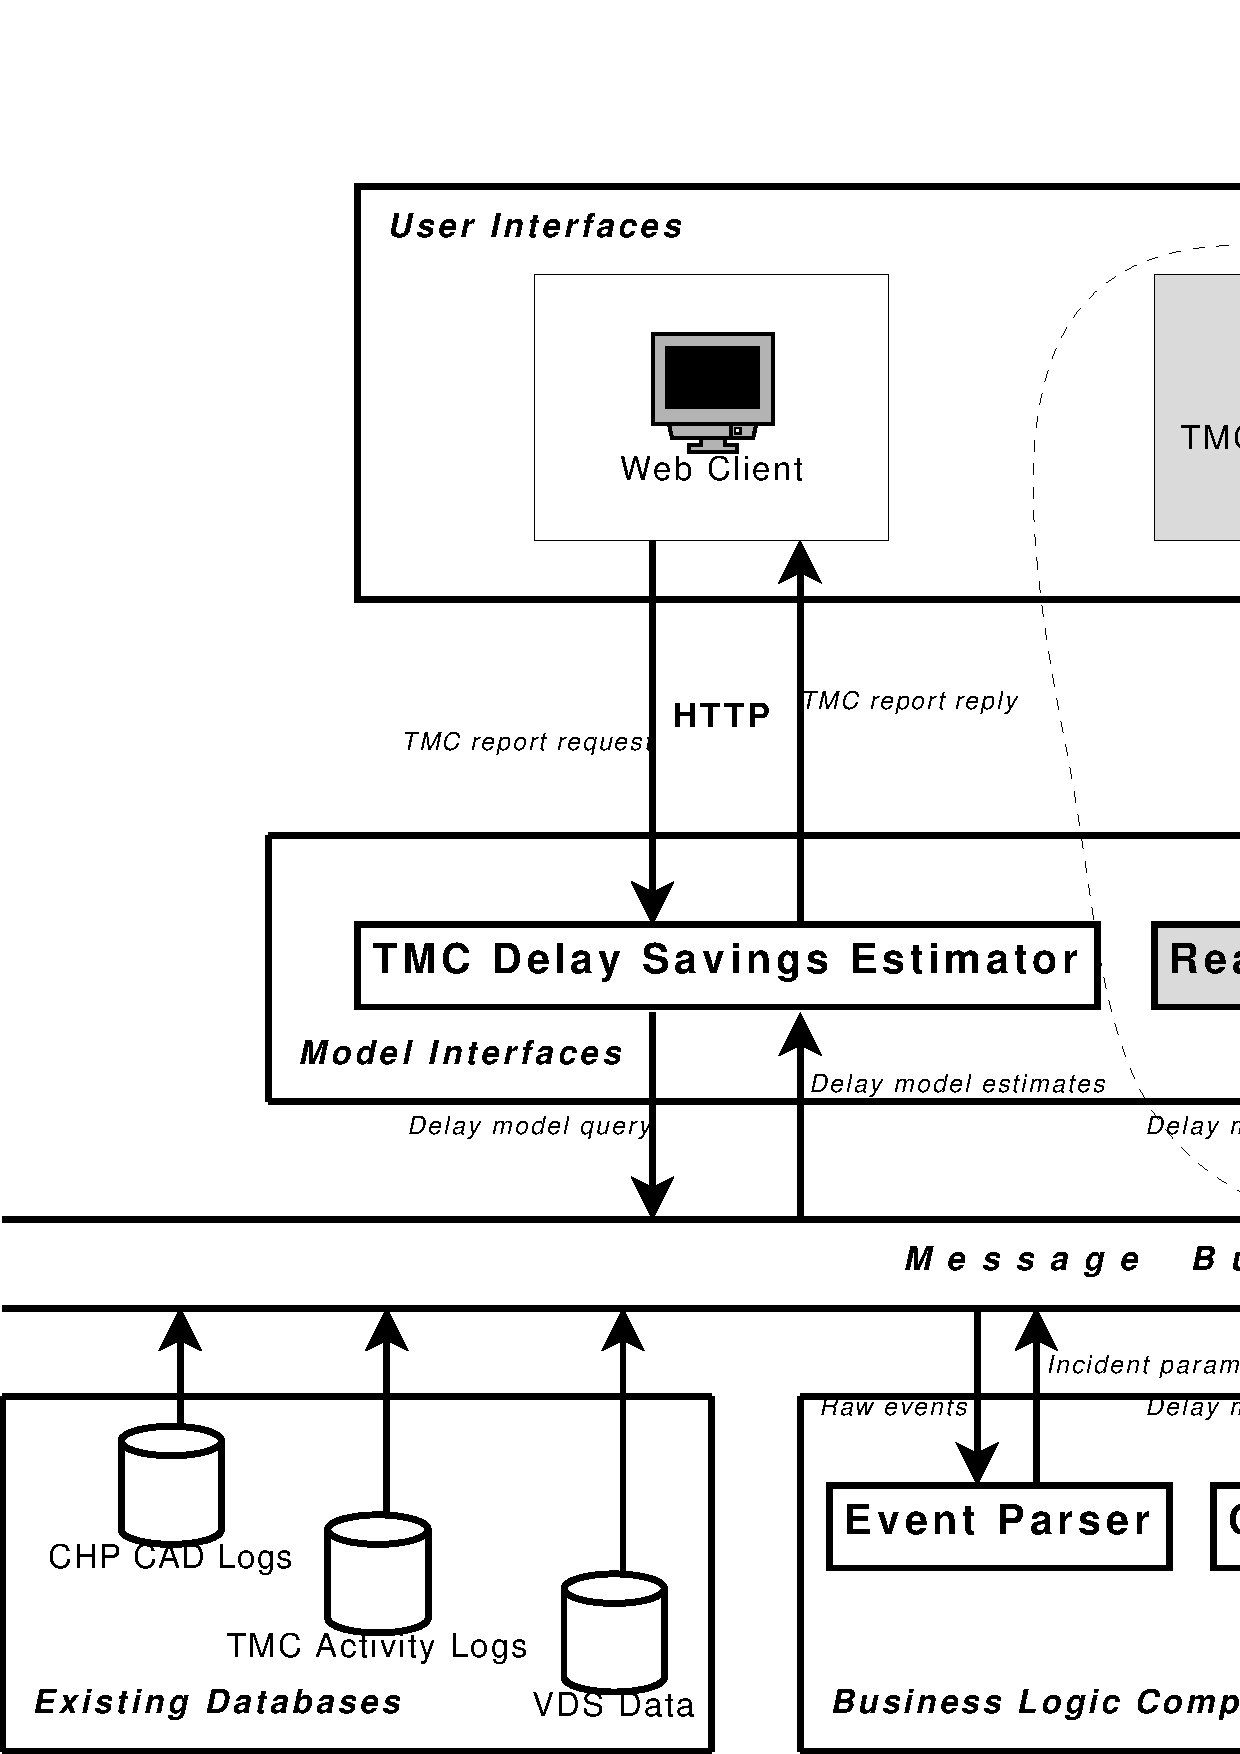
\includegraphics[width=\textwidth]{figs/software-arch.png}
    \inputTikZ{figs/status}
    \caption{System architecture of the TMC performance evaluation
      system.  \fixme{crindt}{Show only functional}}
    \label{fig:system-arch}
  \end{center}
\end{figure}

We discuss each of these components in the following sections.


\section{Databases}
\label{sec:databases}

\subsection{TMC activity data}
\label{sec:activity-data}

The first interim report for this project
\citep{rindt08:_measur_based_system_for_tmc_perfor_evaluat} we noted
that
\begin{quote}
  The \ac{D12} \ac{TMC} activity log records sufficient \ac{TMC} activity to perform
  the basic delay calculation and evaluate a limited portion of the
  benefits provided by the \ac{TMC}. For the activity log to be more
  generally useful to performance evaluation, entries in the log
  should be tied both to specific technologies that offer notable
  impacts on \ac{TMC} processes or to procedures that are designed to have
  intended effects.
\end{quote}
These recommendations were folded into a set of modifications made to
the \ac{D12} \ac{TMC} activity log application under UCI subaward \#2009-2291
between Caltrans \ac{D12} and UCI.  The details of this work is included in
Appendix A.  The most signficant changes with respect to the \ac{TMCPE}
analysis is that the activity log was modified to:
\begin{itemize}
\item log the specific critical events outlined in
  chapter~\ref{chap:tmc-activity};
\item embed the data from the \ac{CHP} \ac{iCAD} log (see
  section~\ref{sec:chp-icad-log}) in the activity log database to
  provide a range of additional event information---most notably a
  geocoded location for the incident previously absent from the event
  dataset; and
\item include the data from the \ac{TMC} Radio Communications logs (RLOG),
  which offer additional information about resource allocation during
  incident management.
\end{itemize}

In order to shield the production database from unnecessary loads from
\ac{TMCPE} users, the development team decided to mirror the \ac{TMC}
activity log database to a secure \ac{CTMLabs} server.  This mirror is
further processed during \ac{TMCPE} analysis to remove any sensitive
data such as phone numbers.  Consequently, the web application has no
access to the raw sensitive data of the source database.


\subsection{PeMS 5 minute database}
\label{sec:pems-5-min}

The \ac{TMCPE} service depends on the availability of 5-minute speed
and volume data for each section of roadway being analyzed.  Though
\ac{CTMLabs} has multiple sources for this data (see
section~\ref{sec:system-data}), the team concluded that the \ac{PeMS}
dataset was the most reliable.  The \ac{CTMLabs} deployment therefore
mirrors the \ac{PeMS} ``value-added reseller'' (VAR) feed, which
provides 5-minute section speeds and volumes.  These are mirrored onto
the \ac{CTMLabs} dataserver at 5 minute intervals and are loaded into
the \ac{CTMLabs} \ac{PeMS} database.

In addition to the 5-minute speeds and volumes, the \ac{TMCPE} delay
calculation requires the computation of the expected distribution of
flow and speed for affected sections by time-of-day and day-of-week.
This is computed using a rolling 52-week horizon as described in
equation~(\ref{eq:nominal-speed-obs}).  Since this is a relatively
expensive computation, it is performed only once on demand the first
time an analysis needs it, and then is cached in the database local
\ac{PeMS} database.  A saved query, or 'view' is stored in the database
that automatically selects the distribution from the cache, if
available, or triggers the computation of a new distribution if it is
missing.  This caching improves the performance of the web application
signficantly.


\subsection{TMCPE application database}
\label{sec:tmcpe-app-database}

All domain data generated by the \ac{TMCPE} application are stored in
the application database.  This includes all incident analyses and
their components (such as individual facility analyses).  For
development purposes, the generation of these databases is handled
automatically by the Hibernate persistence system
\citep{king10:_hiber_relat_persis_idiom_java} built into the
\fixme[grails]{crindt}{first mention} framework
\citep{rocher09:_grail_framew_refer_docum} used to deploy the
\ac{TMCPE} application and its services.  The next section discusses
these in more detail.


\section{Components}
\label{sec:components}

The main components of the performance evaluation system fall into two
categories: business logic components that process data to produce new
metrics for use in the \ac{TMC} and interface components that expose
that data to other software or to users in the \ac{TMC}.


\subsection{Business Logic}
\label{sec:logic}

Except where noted, the core business logic is executed via scheduled
services.  The core analysis is scheduled to run daily at 2am to
process the events of the previous day and make them available for
users.

\subsubsection{Incident impact service}

This component encapsulates the incident impact model described in
section~\ref{sec:incident-impact-model}.  It only requires the
activity log ID as input and will automatically query the sensor
database and \ac{CHP} \ac{iCAD} data to obtain further data necessary
for the analysis.  The service returns a list of impacted sections and
associated delay calculations.

The core models for the incident impact service have been developed
using a program written in the \texttt{perl} scripting language
\citep{FIXME}.  The high-level logic for this service is shown in
figure~\ref{fig:inc-imp-serv}.
\begin{figure}[t]
  \centering
  \begin{enumerate}
  \item {\sc \textbf{Obtain Event Data}}: Query activity log database
    for unanalyzed events since last run
  \item {\sc\textbf{Preprocess Events}}: For each unanalyzed event
    \begin{enumerate}
    \item Loop over the activity and communications logs and:
      \begin{itemize}
      \item determine the \fixme[event type]{crindt}{discuss}
      \item import privacy scrubbed data into the application database
      \item identify performance measures information needed to
        formulate the delay calculation.
      \item Use \ac{iCAD} geocoding (where available) and activity log
        location strings to identify the approximate time-space
        location of the event's impact on the
        system.\fixme{crindt}{Discuss this in more detail}
      \item Create a \ac{TMCPE} event object representing the event and
        store it in the database
      \end{itemize}
    \end{enumerate}
  \item {\sc\textbf{Compute Incident Impact}}: For each \ac{TMCPE} event object
    \begin{enumerate}
    \item Using the geocoded location of the approximate event site and
      the critical incident management events from the activity log,
      \fixme[estimate the maximum time-space bounds]{crindt}{more
        detail} of the event on primary and secondary facilities
    \item Query the \ac{PeMS} mirror database for observed speeds and flows
      for the maximum time-space impact region.
    \item Generate the mathematical program that estimates the range
      of incident impact
    \item Send the program to the \fixme[GAMS
      service]{crindt}{explain} to be solved.
    \item Parse the results of the GAMS solution back into the \ac{TMCPE}
      domain classes for use by the \acp{API}
    \end{enumerate}
  \end{enumerate}
  \caption{Incident impact service procedural logic}
  \label{fig:inc-imp-serv}
\end{figure}
It involves three main steps: obtaining raw event data from all data
sources, pre-processing that data to identify the critical incident
management events, and computing the incident and TMC impacts.

\paragraph{Recommendations for future improvements}

A custom solver could be designed with additional work to solve the
mathematical program for the delay calculations more efficiently.

We have also engaged data mining experts to develop improved
statistical techniques for providing congestion evidence for the delay
calculation in section~\ref{sec:delay-calc}.


\subsubsection{TMC impact service}
\label{sec:tmc-impact-service}
The \ac{TMC} impact service encapsulates the \ac{TMC} impact model resulting
from the work described in section~\ref{sec:mod-tmc-impacts}.  This
service requires as input the activity log ID of the incident to be
analyzed, the output from the incident impact service in order to
characterize the critical section and estimate the arrival pattern to
the impacted region, and any parameters characterizing changes to the
observed incident response As with the incident impact service, this
model independently accesses additional databases as necessary to
support its analysis.  The service updates the \ac{TMCPE} domain classes
for the event to include the estimated delay savings attributable to
actions characterized by the input parameters.

\fixme{crindt}{flesh this out some.  Probably just collapse with the
  above section.}



\subsection{Interfaces}
\label{sec:interfaces}

The core logic generates data objects that can be adapted for the
use-cases described in section~\ref{sec:use-cases}.  To support these
applications, the architecture includes two main interfaces to the
core logical services.  

\subsubsection{Web-based incident post-analysis tool}

The primary interface to the performance evaluation system is a
map-based web interface that allows an analyst to query the model for
\begin{itemize}
\item \ac{TMC} benefits (delay savings) for specific incidents
\item \ac{TMC} benefits for a set of incidents meeting particular criteria
  (location, time of day, severity, etc.)
\end{itemize}
The interface will gives analyst control of relevant input parameters
to the model, but assumes sensible defaults where possible.

The system uses a web-based interface built atop the grails framework,
which is an open-source java-based web application system that is
compatible with existing projects in \ac{CTMLabs}.  Within that framework,
we are implementing a map-based interface using the OpenLayers
\texttt{javascript} library \citep{openlayers} and the OpenStreetmap map image
tiles \citep{openstreetmap} (google maps can also be used as a
background layer).

Analysis of a particular incident is reflected in the analysis of all
potentially impacted facilities, whose estimated time-space impacts
are displayed using a custom \texttt{javascript} widget developed for
this project.  Additional detail of the user interface is provided in
chapter~\ref{chap:user-guide}.

% \subsubsection{Incident status event channel}

% To support other use-cases involving integration of the incident delay
% model into \ac{TMC} operations or other external services, we will provide
% an event channel and associated external interface (using, e.g., SOAP
% or other web-based data feed technology) over which estimates from the
% core delay model will be broadcast to any subscribers.  These
% estimates, for instance, might be integrated into \ac{TMC} processes (and
% associated software) in order to prioritize incident response being
% managed by the \ac{TMC}.

% \paragraph{STATUS:} No work has been completed on the status event channel.


\subsubsection{CTMLabs API}
\label{sec:ctmlabs-api}

As part of its integration into the \ac{CTMLabs} architecture, the
\ac{TMCPE} analyses are offered as a using the \ac{REST} style of
exposing services on the Internet
\citep{fielding00:_archit_styles_desig_networ_softw_archit} using the
CTMLabs \ac{API}.

The RESTful endpoint is authenticated using the \ac{CAS} server
deployed in the \ac{CTMLabs} and returns data formatted as
\ac{GeoJSON} objects \citep{butler08:_geojs_format_specif} as shown in
figure~\ref{fig:ctmlabs-api}\footnote{Technically, the \ac{API} uses a
  \texttt{javascript} pattern known as \ac{JSONP}
  \citep{özses09:_cross_jsonp_part} to avoid problems introduced by
  the \emph{same origin policy} enforced by web browsers.
  Effectively, however, the \ac{API} requires the affiliated
  website---\ac{TMCPE} in this case---to return a JSON object as
  described.}.  In the \ac{TMCPE} implementation of this \ac{API}, the
\texttt{memo} field is filled with the CAD id of the event in
question, the \texttt{locString} field with the facility and direction
of the affected section, and the \texttt{url} field with a link back
into the RESTful \ac{TMCPE} page for the associated analysis.
\begin{figure}[t]
  \centering
\begin{singlespace}
\begin{verbatim}
{ "type": "FeatureCollection",
  "features": [
    { "type":           "Feature",
      "id":             <appid>,         // optional
      "geometry":       <geojson geometry object>,
      "properties":    
         { "locString": <string describing location>,
           "memo":      <string describing data>,
           "url":       <link back to application url for this object>,
         }
    },
    { "type": "Feature"
      ...
    },
    ...
  ]
}
\end{verbatim}
\end{singlespace}
\caption{CTMLabs API format}
  \label{fig:ctmlabs-api}
\end{figure}

Using this \ac{API}, the \ac{TMCPE} application has been integrated into the
\ac{CTMLabs} project interface, which shows the extent of the \ac{TMCPE} data
available, but does not expose the underlying details to
unauthenticated users.
\fixme{crindt}{Project interface picture}

\subsubsection{Interface security}
\label{sec:interface-security}

Access to the data on either of the above interfaces requires that the
user logs in to the \ac{CTMLabs} \ac{CAS} server to initiate a
session.  Only those \ac{CTMLabs} users that have been added to the
\ac{TMCPE} group on the \ac{CTMLabs} \ac{LDAP} server are permitted
access to the \ac{TMCPE} data.  All interfaces use secure sockets over
the HTTP protocol (HTTPS) to encrypt data over the Internet.

\subsection{Physical deployment of TMCPE Application}
\label{sec:arch}

The logical system architecture described above is designed to
leverage existing software under development for related research
being carried out in the \ac{CTMLabs}.  The tasks necessary to deploy the
\ac{TMC} Performance Evaluation platform using this architecture are
confined to the specification of the data sources, business logic
(software implementing the models described in
chapter~\ref{sec:method}), user interfaces, and information flows
between those components.

\fixme{crindt}{Insert as-built about here and discuss}



\fixme{crindt}{%
  Discuss portability somewhere around here---don't forget to mention
  TMCAL.  Things to note:
  \begin{itemize}
  \item CAS integration would need to be rolled back (minor)
  \item Help system not integrated (minor)
  \item Requirement for a GAMS license
  \item Database requirements
    \begin{itemize}
    \item PeMS data
    \item Activity data (incl. steps to interface with TMCAL or similar)
    \item use of map tiles
    \end{itemize}
  \end{itemize}
}



\chapter{Representative results}
\label{chap:results}

\begin{itemize}
\item Discuss performance/processing, etc
\item General statistics (total incidents, types, etc.)
\item Discuss how the delay method differs
  \begin{itemize}
  \item Max speed threshold
  \item Capturing of more delay, not just D35
  \item Accounting for spectator slowing
  \item Accounting for network effects (not complete)
  \end{itemize}
\end{itemize}

\chapter{Conclusion}
\label{chap:conclusion}






%\includegraphics[width=\textwidth]{images/inc-61-ss.png}

%\printnomenclature 


\appendix

\chapter{Summary of Work Performed Under UCI Subaward \#2009-2291}
\label{chap:actlog-sub}

\clearpage

%% This 
\includepdf[pages={1-9},pagecommand={\thispagestyle{plain}},trim=0in 1in 0in 1in,clip]{AL_Summary_Report_9-10.pdf}

\clearpage


\chapter{Using the web application}
\label{chap:user-guide}

\fixme{crindt}{Link to the use cases (section~\ref{sec:use-cases}.)}

\section{Interface basics}
\label{sec:ui-basics}

\subsection{Logging in}
\label{sec:ui-login}

\begin{figure}[t]
  \begin{center}
    \includegraphics[width=\textwidth]{images/ctmlabs-login.png}
    \caption{The CTMLabs CAS login screen}
    \label{fig:ctmlabs-login}
  \end{center}
\end{figure}

\fixme{crindt}{Discuss the log in process and the integration with the
  CAS server.  include screenshots}

\subsection{Menus and status}
\label{sec:ui-menu}


\begin{figure}[t]
  \begin{center}
    \includegraphics[width=\textwidth]{images/tmcpe-menu.png}
    \caption{The TMCPE menus}
    \label{fig:tmcpe-menu}
  \end{center}
\end{figure}


\subsection{Getting help}
\label{sec:ui-help}

\begin{figure}[t]
  \begin{center}
    \includegraphics[width=\textwidth]{images/tmcpe-main-help.png}
    \caption{The TMCPE help screen.}
    \label{fig:tmcpe-main-help}
  \end{center}
\end{figure}

\fixme{crindt}{Note that help resides on the project interface.  This is a portability issue.}

\subsection{Reporting problems}
\label{sec:ui-prob}

\begin{figure}[t]
  \begin{center}
    \includegraphics[width=\textwidth]{images/tmcpe-report-problem.png}
    \caption{Reporting a problem with the TMCPE application.}
    \label{fig:tmcpe-report-problem}
  \end{center}
\end{figure}

\fixme{crindt}{Discuss link to \url{http://tracker.ctmlabs.net}}


\section{Querying for specific data}
\label{sec:ui-query}

\begin{figure}[t]
  \begin{center}
    \includegraphics[width=\textwidth]{images/tmcpe-query.png}
    \caption{The TMCPE query pane.}
    \label{fig:tmcpe-query}
  \end{center}
\end{figure}

\fixme{crindt}{Query options and how to use them.  Note any quirks.}

\paragraph{Time Options}

\paragraph{Incident Options}

\paragraph{Other Options}




\section{Viewing query results}
\label{sec:ui-viewing}

\begin{figure}[t]
  \begin{center}
    \includegraphics[width=\textwidth]{images/tmcpe-query-screen.png}
    \caption{The query screen.}
    \label{fig:tmcpe-1}
  \end{center}
\end{figure}


\subsection{Map view}
\label{sec:ui-summary-stats}

\fixme{crindt}{Map legend.}

\subsection{Summary statistics}
\label{sec:ui-summary-stats}

\section{Analyzed event detail}
\label{sec:ui-analyzed-event-detail}

\begin{figure}[t]
  \begin{center}
    \includegraphics[width=\textwidth]{images/tmcpe-1.png}
    \caption{The incident detail view.}
    \label{fig:tmcpe-1}
  \end{center}
\end{figure}


\fixme{crindt}{Map, TSD, interactions between them, etc.}


\clearpage

\chapter{Acronyms}
\begin{acronym}[CTMLabs]
  \acro{ATMS}{Advanced Transportation Management System}
  \acro{TMC}{Transportation Management Center}
  \acro{PeMS}{Performance Measurement System}
  \acro{TMCPE}{\acs{TMC} Performance Evaluation}
  \acro{CAS}{Central Authentication System}
  \acro{CTMLabs}{California Traffic Management Laboratories}
  \acro{LDAP}{Lightweight Directory Access Protocol}
  \acro{API}{Application Programming Interface}
  \acro{CHP}{California Highway Patrol}
  \acro{iCAD}{Intelligent Computer Aided Dispatch}
  \acro{CMS}{Changeable Message Sign}
  \acro{RMS}{Ramp Metering Station}
  \acro{HAR}{Highway Advisory Radio}
  \acro{UCI}{University of California, Irvine}
  \acro{D12}{Caltrans, District 12}
  \acro{TMCAL}{Traffic Management Center Activity Logging}
  \acro{TMT}{Traffic Management Team}
  \acro{HAZMAT}{HAZardoes MATerial}
  \acro{REST}{REpresentational State Transfer}
  \acro{GeoJSON}{Geographic JavaScript Object Notation}
  \acro{JSONP}{JavaScript Object Notation with Padding}
\end{acronym}


\bibliographystyle{apalike}
\bibliography{refs}

\end{document}
